%%
%% Computers & Geosciences submission manuscript (cas-sc).
%% Body ported from 02_arXiv_Paper/main.tex (arXiv:2604.22721).
%%
%% Class/style: local Elsevier CAS bundle v2.4 (2024/05/04)
%%   ./cas-sc.cls, ./cas-common.sty, ./cas-model2-names.bst
%% Full vendor snapshot: ../els-cas-templates/
%% CAGEO journal checklist reference: ../CAGEO_LaTeXTemplate/
%%
%% cas-sc already loads: graphicx, amsmath/amssymb/amsfonts, booktabs, hyperref (url).
%%%%%%%%%%%%%%%%%%%%%%%%%%%% SUBMISSION CHECKLIST %%%%%%%%%%%%%%%%%%%%%%%%%%%%
%% _ Highlights
%% _ Authorship statement (CRediT via \credit + \printcredits)
%% _ Single column and double spaced
%% _ Author-date references
%% _ Code availability section
%% Cover letter: prepare separately for Editorial Manager if required.
%% * Manuscripts that do not meet journal guidelines may be desk-rejected.
%%%%%%%%%%%%%%%%%%%%%%%%%%%%%%%%%%%%%%%%%%%%%%%%%%%%%%%%%%%%%%%%%%%%%%%%%%%%%%

\documentclass[a4paper,fleqn]{cas-sc}

\usepackage[authoryear,sort&compress]{natbib}
\usepackage{setspace}
\usepackage{lineno}
\usepackage{placeins} % Targeted barriers at workload transitions.
\usepackage{needspace} % Keep response definitions with their equations.
\linenumbers

% Formal math notation (vectors bold italic; matrices/arrays bold roman)
\newcommand{\vect}[1]{\boldsymbol{#1}}  % physical/algebraic vectors
\newcommand{\mat}[1]{\mathbf{#1}}       % matrices / 2-D array operands

\begin{document}
\let\WriteBookmarks\relax
\def\floatpagepagefraction{1}
\def\textpagefraction{.001}

\shorttitle{Spectral-Domain Local Statistics}
\shortauthors{Valdivia et al.}

\title[mode = title]{Spectral-Domain Local Statistics with Missing-Data Support for Cartesian and Polar Grids}
\tnotemark[1]
\tnotetext[1]{A preprint of this manuscript is available as arXiv:2604.22721.}

\author[1]{Jairo M. Valdivia}[orcid=0000-0003-0709-1163]
\cormark[1]
\ead{jairo.valdiviaprado@colorado.edu}
\credit{Conceptualization, Methodology, Software, Validation, Formal analysis, Writing -- original draft}

\author[1]{William E. Chapman}[orcid=0000-0002-0472-7069]
\ead{william.chapman@colorado.edu}
\credit{Methodology, Writing -- review \& editing}

\author[1]{Katja Friedrich}[orcid=0000-0001-8417-4232]
\ead{katja.friedrich@colorado.edu}
\credit{Supervision, Writing -- review \& editing}

\affiliation[1]{organization={Department of Atmospheric and Oceanic Sciences, University of Colorado Boulder},
            city={Boulder},
            state={CO},
            country={USA}}

\cortext[1]{Corresponding author}

\begin{abstract}
We present an integrated spectral method for computing local mean, variance, and standard deviation on Cartesian and polar grids with missing data. The method combines discrete cosine and fast Fourier transforms with missing-data normalization, allowing the kernel, width, and reflective or periodic boundary condition to be selected independently for each axis. For polar grids, range-dependent angular filter widths are incorporated directly into the spectral calculation, avoiding explicit spatial-convolution loops over individual range gates. Tests with incomplete one-dimensional signals, two-dimensional radar observations, and three-dimensional Cartesian wind fields show close numerical agreement with weight- and boundary-matched reference calculations. On the tested radar sweep, spectral Gaussian statistics were approximately 45--48 times faster than the spatial Gaussian convolution baseline. For three-dimensional Cartesian grids, prepared spectral computation of all three statistics was up to 47 times faster than NumPy window reductions, 40 times faster than Astropy direct convolution, and five times faster than Astropy FFT convolution, with the largest gains for wider windows. The framework is supported by the Python library \texttt{dct\_toolkit} and accompanying experiment scripts.
\end{abstract}

%% Legacy graphical abstract omitted: mislabeled mask response and obsolete denominator normalization.

%% Highlights: Elsevier requires a separate editable file for EM upload
%% (see highlights.txt). Do not embed a highlights environment here.

\begin{keywords}
spectral filtering \sep normalized convolution \sep boundary conditions \sep local statistics \sep missing data \sep polar coordinates
\end{keywords}

\maketitle

\doublespacing

%% ========================================================================
\section{Introduction}
\label{sec:introduction}

Large gridded datasets in meteorology, radar remote sensing, Earth observation, and related scientific imaging workflows
routinely contain missing or invalid values due to cloud contamination, quality-control masking, beam blockage, clutter
filtering, and acquisition geometry  \citep{JuRoy2008,Shen2015,Hubbert2009Part1}.
In these workflows, local mean, variance, and standard deviation are foundational
diagnostics for smoothing and quality control, but their calculation must distinguish missing values from measured zeros and account for the available data in each neighborhood.

Local statistics can be computed using convolution, which combines neighboring values according to weights defined by a kernel. The kernel’s shape and width determine how observations contribute to the calculation. When data are missing, normalized convolution accounts for the available observations by filtering the data and a validity mask separately, then dividing the filtered data by the filtered mask \citep{Knutsson1993,Westin1994,Pham2006}. In scientific software, Astropy provides \href{https://docs.astropy.org/en/v8.0.2/api/astropy.convolution.convolve.html}{mask-aware convolution} with normalization over available observations \citep{Astropy2022}.
Convolution can be performed directly in the spatial domain or using spectral transforms. For $N$ grid cells and a kernel with $K$ entries, generic direct convolution requires $\mathcal{O}(NK)$ operations, whereas applying a prepared fast-transform filter typically requires $\mathcal{O}(N\log N)$ operations \citep{Cooley1965,Oppenheim1999,Nussbaumer1982}. This makes spectral filtering attractive for wide kernels, although specialized spatial algorithms can be faster for some kernels and implementations \citep{Smith1997}. Near the edges of a grid, a kernel can extend beyond the available data, so the calculation must specify how to treat the boundary. In the spatial domain, one option is to truncate the window at the edge and normalize using only the values inside the grid. Other choices extend the data beyond the grid. Periodic boundaries treat opposite edges as neighbors, while reflective boundaries mirror values at the edges. In spectral convolution, the transform and any padding determine the boundary treatment. The discrete cosine transform (DCT) \citep{Ahmed1974,Makhoul1980} provides a spectral approach compatible with reflective boundaries \citep{Strang1999,Ng1999,Martucci1994}. In contrast, FFT-based convolution without appropriate padding imposes periodic boundaries.

The appropriate kernel width and boundary treatment also depend on grid geometry. In radar data, the distance between adjacent rays increases with range, so a fixed angular window covers a changing physical width \citep{Bringi2001,Fabry2015}. \citet{Valdivia2026RadarDCT} developed a spectral method for radar smoothing with range-dependent angular widths. In their radar application, missing values were filled by interpolation before smoothing, and the filled values contributed to the result. Calculating local mean and variability directly from available observations therefore requires missing-data handling to work together with the boundary conditions and range-dependent polar filter. More generally, an integrated method is needed to calculate these statistics on incomplete N-dimensional Cartesian and polar grids.

We present a spectral framework for calculating local mean, variance, and standard deviation on Cartesian and polar grids with missing data. By combining the polar filtering approach with normalized convolution, the framework calculates these statistics directly from the available observations without first filling missing values. The user can choose the kernel, width, and reflective or periodic boundary independently for each filtered axis. The framework also supports regular polar arrays with additional axes, such as time or elevation, and is implemented in the Python library \texttt{dct\_toolkit}. We evaluate the framework using one-dimensional signals, a real two-dimensional radar sweep, and a synthetic three-dimensional Cartesian wind field. Figure~\ref{fig:statistics_pipeline} summarizes the direct calculation used in the validation.

\begin{figure}[htbp]
	\centering
	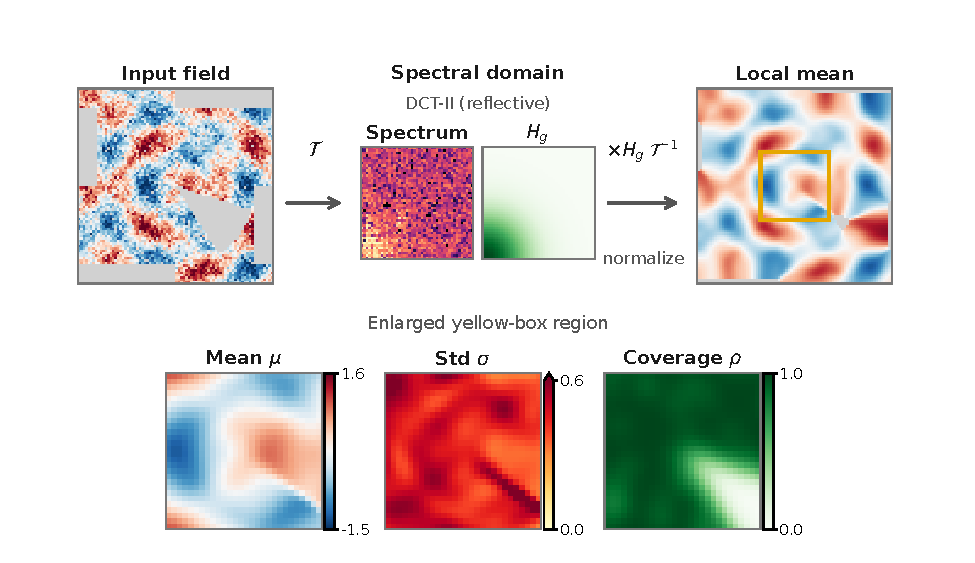
\includegraphics[width=\linewidth]{figures/round1/v2.0.0/visual_pipeline/pdf/visual_statistics_pipeline.pdf}
	\caption{Direct local statistics illustrated on an incomplete synthetic two-dimensional Cartesian field. Gray marks missing inputs and undefined estimates. The spectrum is that of the zero-filled input; the full sampled Gaussian default in v2.0.0 uses reflective boundaries on both axes. The same filter is applied to the valid data, their squares, and the original validity mask. The filtered mask normalizes the moments and gives local data coverage $\rho$. The enlarged panels show the yellow-box region. Input and mean colors use the input's 1st--99th percentile range; the standard-deviation scale saturates above its upper limit. Moment estimates are undefined where the filtered mask is nonfinite or at most $10^{-3}$; default completion is not used. Section~\ref{sec:nc_statistics} defines the quantities and their interpretation.}
	\label{fig:statistics_pipeline}
\end{figure}

Section~\ref{sec:convolution_theorem} defines filters and geometry, and Section~\ref{sec:nc_statistics} formulates local statistics. Section~\ref{sec:software_implementation} describes the software implementation, Section~\ref{sec:validation} presents numerical evaluation and applications, and Section~\ref{sec:performance} reports computational measurements. Sections~\ref{sec:discussion} and \ref{sec:conclusion} discuss limitations and conclude.

\FloatBarrier
%% ========================================================================
\section{Spectral methods for Cartesian and polar grids}
\label{sec:convolution_theorem}

In this paper, a filter is an operation that combines values along one
or more grid axes according to specified spectral responses and
boundary conditions. An individual filtering stage can have a
convolution interpretation. A complete filter may combine several
stages in a prescribed order, as in the range-dependent polar method.

\subsection{Grids and notation}
\label{sec:notation}

Let \(x\) be an observed field on a regular \(D\)-dimensional tensor grid, with multi-index \(\mathbf{i}=(i_1,\ldots,i_D)\) and axis lengths \(N_a\), where \(i_a=0,\ldots,N_a-1\). The binary validity mask \(m(\mathbf{i})\) is one for finite observations retained as valid and zero for missing or excluded observations. Missing-value markers and observations excluded by instrument flags or other quality-control criteria have \(m(\mathbf{i})=0\). Define \(x_m\) and \(x_m^{(2)}\) by copying valid values of \(x\) and \(x^2\), respectively, and replacing invalid entries with zero. Invalid values are replaced explicitly by zero rather than multiplied by the mask; valid values and their squares must be representable as finite inputs.

The filter can be applied along some or all axes of the grid. We denote the set of selected axes by \(\mathcal F\); data slices indexed by the remaining axes are processed independently. For each selected axis \(a\), the operator \(K_a\) filters the field along that axis using its specified kernel response, width, and boundary condition. The complete filter \(\mathcal S_g\) combines the selected axis filters. For fixed geometry, kernel choices and widths, and boundary conditions, \(\mathcal S_g\) is linear. Section~\ref{sec:nc_statistics} applies the same complete filter to \(x_m\), \(x_m^{(2)}\), and \(m\) before normalizing the moments.

The kernel specification $g$ selects Gaussian, analytical boxcar, or odd discrete boxcar independently on each filtered axis. Widths $W_a$ are finite, positive, and expressed in grid cells; the polar conversions below may make them depend on range or elevation, but not on position along the line being filtered. A reflective or periodic boundary condition is prescribed for each filtered axis. Table~\ref{tab:notation} summarizes the filtering symbols and local-statistics quantities used subsequently.

\begin{table}[htbp]
	\centering
	\caption{Summary of notation.}
	\label{tab:notation}
	\begin{tabular}{@{}p{0.26\linewidth}p{0.68\linewidth}@{}}
		\toprule
		Symbol                   & Meaning                                                    \\
		\midrule
		$x$, $m$ & observed field and binary validity mask \\
		$\mathbf{i}$, $D$ & grid multi-index and number of array dimensions \\
		$x_m$, $x_m^{(2)}$ & valid data and squared data, zero-filled at invalid positions \\
		$\mathcal{F}$, $a$, $N_a$ & filtered-axis set, axis index, and axis length \\
		$k_a$, $\omega_{a,k_a}$ & represented frequency index and angular frequency in radians per grid cell \\
		$g$, $H_{g,a}$ & kernel specification and axis-wise spectral response \\
		$W_a$, $M_a$, $\sigma_{g,a}$ & converted grid width, odd discrete width, and Gaussian bandwidth \\
		$\ell$ & integer offset from the kernel center along axis $a$, in grid cells \\
		$g_a[\ell]$, $q_a$ & normalized Gaussian samples and integer kernel radius \\
		$K_a$, $\mathcal{S}_g$ & one filtering stage and the complete smoothing operator \\
		$R_j$, $\theta$, $\phi$, $\eta$ & actual range, angular coordinate, azimuth, and elevation \\
		$L_a$, $\Delta_a$ & requested physical width and coordinate spacing on axis $a$ \\
		$d$, $\rho$ & raw mask response $\mathcal{S}_g\{m\}$ and local data coverage \\
		$\mu$, $M_2$ & normalized first and second raw moments \\
		$\sigma^2$, $\sigma$ & reported local variance and standard deviation \\
		$N_{\mathrm{eq}}$, $A$ & equivalent data count $A\rho$ and nominal grid-unit window factor \\
		$N_{\mathrm{ESS}}$ & statistical effective sample size \\
		$\epsilon$, $\bar{x}$ & denominator threshold (default $10^{-3}$) and completed first-moment field \\
		$\vect{v}$ & wind vector field with components $u,v,w$ \\
		$\mat{X}$, $\mat{Y}$ & polar input and filtered-output arrays \\
		\bottomrule
	\end{tabular}
\end{table}

%% Font convention (not printed): vectors bold italic via \vect; matrices/2-D
%% arrays bold roman via \mat; multi-index \mathbf{i}; scalars and 1-D H_g[k] italic.

\subsection{Boundary-dependent axis filters}

For a finite input field $f$, filtering along axis $a\in\mathcal{F}$ takes the form
\begin{equation}
	K_a\{f\} = \mathcal{T}_a^{-1}\!\left\{\mathcal{T}_a\{f\} \odot H_{g,a}\right\},
	\label{eq:smooth_operator}
\end{equation}
Here, \(\mathcal T_a\) and \(\mathcal T_a^{-1}\) are the forward and inverse transforms along axis \(a\), \(H_{g,a}\) is the selected kernel's spectral response, and \(\odot\) denotes element-wise multiplication. The response is evaluated using the local converted width and is shared along axes on which it does not vary. The transform pair is DCT-II/IDCT-II for reflective boundary conditions or RFFT/IRFFT for periodic boundary conditions, with orthonormal normalization and inverse output length \(N_a\). Spectral multiplication implements the specified boundary-dependent filter, not an unrestricted convolution identity for arbitrary DCT arrays \citep{Oppenheim1999,Strang1999,Martucci1994}.

The boundary model is chosen before filtering from the acquisition geometry and the intended treatment of the domain edges. Under periodic boundary conditions, the two ends of an array are treated as neighbors, as in a complete circular radar sweep with no repeated endpoint. A sector's endpoints are not adjacent; reflective azimuth is one available non-periodic model. Under reflective boundary conditions, values beyond the array are mirrored at its edges. This is a prescribed boundary model, not an estimate of the physical field outside the domain. Internal invalid cells instead have $m=0$ and do not create new reflective interfaces. Observations on either side of a gap can contribute to the same estimate through the prescribed operator. Thus the validity mask excludes observations but does not impose an impermeable physical barrier or automatically partition the domain.

For an orthonormal DCT-II matrix $\mat{C}_a$, the matrix representation of a reflective filtering stage on a fixed line is
\begin{equation}
	\mat{K}_a=\mat{C}_a^{\mathsf{T}}\operatorname{diag}(H_{g,a})\mat{C}_a.
	\label{eq:boundary_operator}
\end{equation}
Here $H_{g,a}$ supplies the filter eigenvalues, not generally the ordinary DCT of sampled kernel values. For a centered symmetric discrete kernel, its cosine response gives convolution under half-sample even extension about the outer cell faces, consistent with the discrete Neumann model \citep{Strang1999,Ng1999,Martucci1994}. The RFFT branch instead implements circular filtering. Table~\ref{tab:frequency_vars} specifies the angular frequencies and represented indices for both modes.

The discrete boxcar has the standard frequency response of a centered moving-average filter \citep[Chap.~15]{Smith1997}. The analytical boxcar extends its sine-ratio expression to positive real widths. For Gaussian convolution, $\ell$ denotes the integer offset from the kernel center along axis $a$, measured in grid cells. In the matched radar comparison, we use samples $g_a[\ell]\propto\exp[-\ell^2/(2\sigma_{g,a}^2)]$ for $\ell=-q_a,\ldots,q_a$, normalized so that $\sum_{\ell=-q_a}^{q_a}g_a[\ell]=1$, with bandwidth $\sigma_{g,a}=W_a/\sqrt{12}$ and radius $q_a=\lceil4\sigma_{g,a}\rceil$.

\Needspace{12\baselineskip}
The spectral responses along axis $a$ are denoted by $H_{\mathrm{box},a}$ for the analytical boxcar, $H_{\mathrm{dis},a}$ for the odd discrete boxcar, and $H_{\mathrm{gauss},a}$ for the sampled Gaussian. The discrete-boxcar width $M_a$ is a positive odd integer. Using the boundary-dependent frequencies in Table~\ref{tab:frequency_vars}, the responses for local grid width $W_a>0$ are

\begin{align}
	H_{\mathrm{box},a}[k_a] & = \frac{\sin(W_a\omega_{a,k_a}/2)}{W_a\sin(\omega_{a,k_a}/2)}, \label{eq:tf_boxcar_analytical} \\*
	H_{\mathrm{dis},a}[k_a] & = \frac{1}{M_a}\left(1+2\sum_{\ell=1}^{(M_a-1)/2}\cos(\ell\omega_{a,k_a})\right), \label{eq:tf_boxcar_discrete} \\*
	H_{\mathrm{gauss},a}[k_a] & = g_a[0]+2\sum_{\ell=1}^{q_a}g_a[\ell]\cos(\ell\omega_{a,k_a}). \label{eq:tf_gaussian}
\end{align}
The analytical-boxcar value at $k_a=0$ is its limit, one. For odd integer $W_a=M_a$, Eqs.~\ref{eq:tf_boxcar_analytical} and \ref{eq:tf_boxcar_discrete} coincide. At other widths, including even integers and fractional values, the analytical response defines a spectral filter rather than an exact centered discrete boxcar. For the analytical boxcar response, widths below one grid cell ($0<W_a<1$) amplify nonzero frequencies rather than smooth them. Section~\ref{sec:filter_implementation} specifies how the implementation selects $M_a$ from $W_a$.

The Gaussian bandwidth $\sigma_{g,a}$ is distinct from the local data standard deviation $\sigma$. The relation $\sigma_{g,a}=W_a/\sqrt{12}$ matches the variances of a continuous Gaussian and a continuous boxcar of width $W_a$. Equation~\ref{eq:tf_gaussian} gives the transfer function of convolution with the sampled Gaussian kernel. It differs from the Fourier response of a continuous Gaussian, $\exp[-(\omega_{a,k_a}\sigma_{g,a})^2/2]$ \citep[Chap.~11]{Smith1997}. Section~\ref{sec:filter_implementation} distinguishes the full sampled Gaussian default from this benchmark cutoff. All responses preserve constants because $H_{g,a}[0]=1$. The sampled Gaussian kernel has nonnegative spatial weights, giving nonnegative variance estimates in exact arithmetic. In contrast, applying the continuous Gaussian Fourier response on a finite grid can produce signed spatial weights and negative variance estimates.

\begin{table}[htbp]
	\centering
	\caption{Frequency conventions for every response in Eqs.~\ref{eq:tf_boxcar_analytical}--\ref{eq:tf_gaussian}. Here $N_a$ is the length of the filtered axis.}
	\label{tab:frequency_vars}
	\begin{tabular}{lccc}
		\toprule
		Boundary & $\omega_{a,k_a}$ & Represented $k_a$ & Transform \\
		\midrule
		Reflective & $\pi k_a/N_a$ & $0,\ldots,N_a-1$ & DCT-II (ortho) \\
		Periodic & $2\pi k_a/N_a$ & $0,\ldots,\lfloor N_a/2\rfloor$ & RFFT (ortho) \\
		\bottomrule
	\end{tabular}
\end{table}

\subsection{Cartesian coordinates}

On a Cartesian grid, suppose the filter response along each selected axis is fixed across the other coordinates. This gives standard separable filtering: the axis filters commute, so their order does not change the complete filter \citep[Chap.~24]{Smith1997}. In the joint transform domain, their responses combine as
\begin{equation}
	H_D[k_1,\ldots,k_D] = \prod_{a\in\mathcal{F}} H_{g,a}[k_a].
	\label{eq:nd_separable}
\end{equation}
The inverse joint transform of the transformed input multiplied by $H_D$ gives the complete filtered field. Section~\ref{sec:nc_statistics} applies this same filter to the zero-filled observations, their squares, and the validity mask before calculating the normalized moments. Kernel families, widths, and boundary conditions can differ among the filtered axes; a separable filter need not be isotropic. On a uniformly spaced Cartesian axis, a physical width $L_a$ corresponds to $W_a=L_a/\Delta_a$ grid cells, where $\Delta_a$ is the coordinate spacing. The coordinate-independent responses required for Eq.~\ref{eq:nd_separable} do not generally hold for the polar composition below. The corresponding toolkit interfaces are summarized in Section~\ref{sec:filter_implementation}.

\subsection{Polar coordinates}
\label{sec:polar}

For a two-dimensional angle--range grid, \citet[Sect.~2.3, Eqs.~(12)--(17)]{Valdivia2026RadarDCT} describe filtering first along the angular coordinate and then along range. Let $\theta$ be the angular coordinate, representing either azimuth or elevation, and let the array shape be $(N_\theta,N_R)$. Let $\Delta_\theta$ be the uniform angular spacing in radians, $R_0$ the range of the first gate, and $\Delta_R$ the uniform range-gate spacing. The range at gate $j=0,\ldots,N_R-1$ is $R_j=R_0+j\Delta_R$.

For a requested physical width $L_\theta$ along the angular direction, the corresponding width in angular bins at range $R_j$ is
\begin{equation}
	W_{\theta,\mathrm{grid}}(R_j)=\frac{L_\theta}{R_j\Delta_\theta}, \qquad R_j>0,
	\label{eq:polar_width}
\end{equation}
while a physical range width gives $W_{\mathrm{range}}=L_{\mathrm{range}}/\Delta_R$ gates. This two-dimensional conversion uses $R_j\Delta_\theta$ for the spacing along the angular coordinate. When an elevation axis is also present, the azimuth conversion includes an elevation-dependent factor, as described below.

The angular stage applies a spectral response whose width varies with range:
\begin{equation}
	\mat{Y}_{\theta} = K_\theta\{\mat{X}\}=\mathcal{T}_{\theta}^{-1}\!\left\{\mathcal{T}_{\theta}\{\mat{X}\}\odot \mat{H}_{\theta}\right\}.
	\label{eq:polar_stage1}
\end{equation}
Each column of $\mat{H}_\theta$ uses that gate's width and the angular-axis frequencies from Table~\ref{tab:frequency_vars}, with $N_a=N_\theta$. Its shape is $(N_\theta,N_R)$ for reflective DCT-II or $(\lfloor N_\theta/2\rfloor+1,N_R)$ for periodic RFFT. After returning to the spatial domain, the range stage uses a shared reflective response $H_R$:
\begin{equation}
	\mat{Y} = K_R\{\mat{Y}_{\theta}\}=\mathrm{IDCT}_R\!\left\{\mathrm{DCT}_R\{\mat{Y}_{\theta}\}\odot H_R\right\}.
	\label{eq:polar_stage2}
\end{equation}
Angular smoothing is performed first so that each range gate is filtered using its own range-dependent angular width. For the physical widths in Eq.~\ref{eq:polar_width}, that width corresponds to the gate's distance from the origin. The range filter then combines the angularly smoothed values from the gates, using the same range response $H_R$ at each angular position. This order preserves the prescribed angular scale of each gate's contribution. The complete operator is $\mathcal{S}_g=K_R\circ K_\theta$; because the angular response varies with range, the stages generally do not commute. The resulting filter is linear and constant-preserving, but is not a single stationary separable 2D convolution. Table~\ref{tab:boundary_modes} gives example boundary interpretations; reflective range is the choice in this construction, not a restriction on all supported filters.

\begin{table}[htbp]
	\centering
	\caption{Example boundary conditions for two-dimensional angle--range filtering. Reflective range boundaries are used in the construction above; periodic range boundaries can also be prescribed. Boundary modes are prescribed, not inferred from the mask.}
	\label{tab:boundary_modes}
	\begin{tabular}{@{}lllp{0.43\linewidth}@{}}
		\toprule
		Axis    & Option     & Transform & Appropriate for                 \\
		\midrule
		Angle   & Reflective & DCT-II    & Angular sector with even endpoint extension \\
		Angle   & Periodic   & RFFT      & Complete circular domain, such as full azimuth, without a repeated endpoint \\
		Range   & Reflective & DCT-II    & Non-periodic range limits used here \\
		\bottomrule
	\end{tabular}
\end{table}

The construction extends to regular N-D arrays with additional axes, such as elevation or time. For an ordered list of selected axes $(a_1,\ldots,a_q)$, the complete filter is
\begin{equation}
	\mathcal{S}_g=K_{a_q}\circ\cdots\circ K_{a_1}.
	\label{eq:nd_polar_operator}
\end{equation}
Axes not selected for filtering index independent domains. An empty selection gives the identity operator. The axis order used in the implementation is specified in Section~\ref{sec:filter_implementation}.

Physical widths on range, time, and linear axes are divided by their coordinate spacings. With elevation $\eta$, the angular conversions are
\begin{equation}
	W_{\mathrm{az,grid}}(R,\eta)=\frac{L_{\mathrm{az}}}{R\cos\eta\,\Delta_\phi}, \qquad
	W_{\mathrm{el,grid}}(R)=\frac{L_{\mathrm{el}}}{R\Delta_\eta}.
	\label{eq:nd_polar_widths}
\end{equation}
The requested widths $L_{\mathrm{az}}$ and $L_{\mathrm{el}}$ are physical distances in the same units as $R$, while $\Delta_\phi$ and $\Delta_\eta$ are angular spacings in radians. The converted widths vary with range; the azimuth width also varies with elevation through $\cos\eta$. These physical conversions require $R>0$, and the azimuth conversion additionally requires $\cos\eta>0$. For a complete circular azimuth grid without a repeated endpoint, $N_\phi\Delta_\phi=2\pi$. A width specified directly in grid cells does not require a physical-coordinate conversion.

The conversions define local coordinate-line scales, not an isotropic Cartesian or geodesic convolution or a cell-volume-weighted average. They support regular named-axis tensor grids, not arbitrary irregular acquisitions or general hyperspherical coordinates.

The nominal grid-unit window factor for the two-dimensional operator is
\begin{equation}
	A_{\mathrm{polar}}(j)=W_{\mathrm{range}}\,W_{\theta,\mathrm{grid}}(j),
	\label{eq:area_polar}
\end{equation}
and more generally $A(\mathbf{i})=\prod_{a\in\mathcal{F}}W_a(\mathbf{i})$, using converted requested widths before discrete-boxcar rounding, not the rounded widths $M_a$. Unfiltered axes contribute no factor. This factor scales the local data coverage in the equivalent data count $N_{\mathrm{eq}}=A\rho$; $A$ is a nominal grid-unit factor, not a physical footprint. The implementation's singleton-axis conventions are given in Section~\ref{sec:filter_implementation}.

The ordered operator in Eq.~\ref{eq:nd_polar_operator} specifies the complete filter used by the statistics in the next section. It acts on each moment input and the mask before a single normalization; normalizing after individual stages generally changes the weights.

%% ========================================================================
\section{Local statistics with missing observations}
\label{sec:nc_statistics}

Normalized convolution accounts for missing observations by filtering the valid data and their validity mask separately, then normalizing the filtered data by the filtered mask \citep{Knutsson1993,Westin1994,Pham2006}. Here we apply the same complete filter $\mathcal{S}_g$ from Section~\ref{sec:convolution_theorem} to the zero-filled observations, their squares, and the original mask. The resulting normalized first and second moments provide the local mean and reported variance, while the filtered mask also supports diagnostics of data availability. The following subsections describe these quantities and their interpretation; Section~\ref{sec:statistics_implementation} describes the toolkit's treatment of insufficient mask response.

\subsection{Weighted local moments}

Let $d(\mathbf{i})=\mathcal{S}_g\{m\}(\mathbf{i})$ be the raw mask response. For a chosen nonnegative threshold $\epsilon$, the direct-ratio calculation accepts only finite $d>\epsilon$ and defines the local mean as
\begin{equation}
	\mu(\mathbf{i}) = \frac{\mathcal{S}_g\{x_m\}(\mathbf{i})}{d(\mathbf{i})}.
	\label{eq:mean}
\end{equation}
The threshold is a strict acceptance test, not an additive term in the denominator. For the reflective Cartesian operator, Eq.~\ref{eq:mean} becomes
\begin{equation}
	\mu(\mathbf{i}) = \frac{\mathrm{IDCT}_D\!\left\{\mathrm{DCT}_D\{x_m\}\odot H_D\right\}(\mathbf{i})}{\mathrm{IDCT}_D\!\left\{\mathrm{DCT}_D\{m\}\odot H_D\right\}(\mathbf{i})}.
	\label{eq:mean_explicit}
\end{equation}

The second raw moment $M_2$ uses the same complete filter and denominator. The reported variance and standard deviation are obtained from the moment difference, clamped from below:
\begin{align}
	M_2(\mathbf{i}) & = \frac{\mathcal{S}_g\{x_m^{(2)}\}(\mathbf{i})}{d(\mathbf{i})}, \label{eq:second_moment} \\
	\sigma^2(\mathbf{i}) & = \max\!\left(0,\,M_2(\mathbf{i})-\mu(\mathbf{i})^2\right), \label{eq:var_clamped} \\
	\sigma(\mathbf{i})   & = \sqrt{\sigma^2(\mathbf{i})}. \label{eq:std}
\end{align}

Write the complete filter as $\mathcal{S}_g\{f\}(\mathbf{i})=\sum_j w_{\mathbf{i}j}f(j)$, where $j$ indexes distinct original observations and $w_{\mathbf{i}j}$ includes all repeated boundary contributions from observation $j$. On the direct-ratio path, nonnegative weights and positive $d$ give normalized valid weights $w_{\mathbf{i}j}m_j/d$ summing to one. The mean is then bounded by the contributing observations, and the raw difference $M_2-\mu^2$ is their nonnegative weighted population variance in exact arithmetic. These are descriptive moments, without a Bessel correction or an unconditional unbiasedness guarantee. Separately completed first- and second-moment fields also lack these direct-ratio guarantees.

Subtracting the squared mean from the second moment can produce small negative values through floating-point cancellation, particularly near zero variance. Equation~\ref{eq:var_clamped} sets these values to zero before taking the square root. For a filter with signed spatial weights, the moment difference can also be negative in exact arithmetic; clamping such a result does not restore the weighted-variance interpretation.

\subsection{Local data coverage and equivalent data count}

For nonnegative, constant-preserving spatial weights, the mask response is
\[
 d(\mathbf{i})=\sum_j w_{\mathbf{i}j}m_j,
 \qquad w_{\mathbf{i}j}\geq 0,
 \qquad \sum_j w_{\mathbf{i}j}=1.
\]
Because $m_j$ is either zero or one, $d(\mathbf{i})\in[0,1]$ is the weighted fraction of available observations. In this case, local data coverage $\rho$ equals $d$. For the equivalent data count, the nominal window factor is
\[
 A(\mathbf{i})=\prod_{a\in\mathcal{F}}W_a(\mathbf{i}),
\]
the product of the requested widths expressed in grid cells along the filtered axes, before discrete-boxcar rounding. Unfiltered axes contribute no factor, and $A$ can vary with position when widths do. The singleton-axis conventions are given in Section~\ref{sec:filter_implementation}. This nominal factor is not necessarily the number of cells in a window. The equivalent data count $N_{\mathrm{eq}}$ scales coverage by $A$:
\begin{equation}
	N_{\mathrm{eq}}(\mathbf{i})=A(\mathbf{i})\rho(\mathbf{i}).
	\label{eq:neff}
\end{equation}
Signed weights can instead place $d$ outside $[0,1]$. The implementation bounds $d$ when reporting $\rho$, as specified in Section~\ref{sec:statistics_implementation}; this yields a bounded diagnostic, not necessarily a fraction or a measure of confidence. Moment normalization always uses raw $d$, and both diagnostics refer to the original mask rather than a mask enlarged by completion.

For a uniform discrete boxcar, $N_{\mathrm{eq}}$ equals the valid-cell count when $A$ matches the actual footprint size $\prod_{a\in\mathcal{F}}M_a$ and boundary extension does not repeat any original observation. In general, including Gaussian weighting and range-dependent polar composition, $N_{\mathrm{eq}}$ is only the bounded mask response expressed on this nominal-width scale, not a count of distinct or independent observations.

Statistical effective sample size, denoted by $N_{\mathrm{ESS}}$, differs from the equivalent data count $N_{\mathrm{eq}}$. For independent observations of equal variance, it is the equivalent number of equally weighted observations whose mean would have the same variance as the weighted mean. For a direct-ratio mean with nonnegative fixed weights and a fixed mask, the squared-weight expression \citep{Kish1992} is
\begin{equation}
	N_{\mathrm{ESS}}(\mathbf{i})=\frac{\left(\sum_j w_{\mathbf{i}j}m_j\right)^2}{\sum_j\left(w_{\mathbf{i}j}m_j\right)^2}.
	\label{eq:weight_ess}
\end{equation}
The weights in Eq.~\ref{eq:weight_ess} must aggregate repeated reflected or wrapped contributions from each distinct original observation before squaring, as in the filter representation above. This quantity generally differs from $A\rho$. Spatial correlation invalidates the independent-observation variance interpretation; neither diagnostic by itself quantifies uncertainty in a geophysical field.

%% ========================================================================
\section{Software implementation}
\label{sec:software_implementation}

The Python library \texttt{dct\_toolkit} implements the filtering and local-statistics framework for Cartesian and polar grids with missing observations. The user specifies a kernel family, a width, and a boundary condition for each filtered axis, and the library applies the complete filter jointly to the data, their squares, and the validity mask before normalizing the moments. Section~\ref{sec:filter_implementation} describes the entry points and the radar benchmark's Gaussian implementation, and Section~\ref{sec:statistics_implementation} describes the diagnostics and the default fallback in \texttt{dct\_toolkit} v2.0.0; Section~\ref{sec:validation} uses direct ratios with completion and restoration disabled.

\subsection{Filter implementation}
\label{sec:filter_implementation}

The release offers two entry points. The reflective Cartesian backend filters all axes with an orthonormal N-D DCT-II pair and accepts widths in grid cells. Mixed reflective and periodic boundaries or a selected subset of Cartesian axes use the explicit-geometry interface with Cartesian directions assigned linear roles, in which every supported kernel accepts either boundary condition on each filtered axis. For a discrete boxcar, the converted width $W_a$ is rounded to the nearest integer with ties to even, raised to at least one, and incremented if even to obtain the odd width $M_a$.

The default \texttt{gaussian} kernel in v2.0.0 uses Gaussian samples at all integer offsets, normalized by their infinite sum. Its transfer function follows Eq.~\ref{eq:tf_gaussian} with the sum extended to infinity and is evaluated to \texttt{float64} precision without a fixed spatial cutoff. This default applies to Cartesian and polar smoothing and statistics, including completion. Figure~\ref{fig:statistics_pipeline} illustrates the default Gaussian kernel.

The radar benchmark uses the same four-standard-deviation cutoff in both implementations to compare equivalent discrete filters. This cutoff is a benchmark setting, not a requirement of spectral filtering. On a fixed grid, the full Gaussian uses the same transform dimensions and filtering passes; its response-preparation costs can differ, and its end-to-end runtime was not measured here.

The benchmark scripts construct the spectral response by accumulating kernel weights on a periodic grid of length $N_a$ for a periodic axis or $2N_a$ for a reflective axis, then transforming the resulting array. The reflective calculation retains the first $N_a$ modes for DCT-II filtering. This construction includes every repeated boundary contribution when the kernel is wider than the axis.

For explicit geometry, each storage axis is assigned an azimuth, elevation, range, time, linear, or batch role, with at most one azimuth, elevation, and range axis. Coordinates, widths, kernel families, width units, and boundary modes are supplied in array order. The selected axes, specified by \texttt{filter\_axes}, are filtered in the fixed role order azimuth, elevation, range, time, then linear, irrespective of storage order; repeated time or linear roles retain array order. By default all non-batch axes are selected, batch axes cannot be selected, and unselected axes index independent domains, including during completion. Singleton axes ($N_a=1$) are identity stages with $W_a=1$.

For the nominal factor $A$, unselected axes contribute no factor and explicit-geometry singleton axes contribute one. The Cartesian backend and index-based polar interface instead retain their requested-width factors even on singleton axes.

Angular coordinates may be supplied in degrees or radians and are converted to radians internally. Without an elevation axis, the azimuth conversion uses a cosine factor of one. Physical and grid-unit widths may be mixed among axes, and neither is capped at the axis length.

Every supplied coordinate vector must be finite and real, match its axis length, and be strictly increasing and uniformly spaced, checked to a relative tolerance of $10^{-6}$. Elevation coordinates after conversion to radians must lie within $[-\pi/2,\pi/2]$. Coordinates are required on selected nonsingleton physical axes and on any range or elevation axis needed for physical angular conversion, even when range or elevation is unfiltered or singleton.

Selected nonsingleton physical angular filters require positive actual ranges; physical azimuth additionally requires $\cos\eta>10^{-12}$ when elevation is present. These checks reject singular origins and azimuthal poles rather than capping widths. For selected nonsingleton physical periodic azimuth, the interface checks $N_\phi\Delta_\phi=2\pi$ with the same $10^{-6}$ relative tolerance, excluding a repeated endpoint. Grid-unit, unselected, and singleton angular filters skip their own physical conversion and these angular checks.

\subsection{Statistics and completion}
\label{sec:statistics_implementation}

The released v2.0.0 moment routines use the direct ratios in Section~\ref{sec:nc_statistics} where the original mask response $d$ is finite and $d>\epsilon$, with $\epsilon=10^{-3}$ by default. At rejected positions, the default \texttt{dct\_mean} routine estimates the mean by completing and smoothing the input field. Let $\bar{x}$ denote this completed field, formed from valid observations in the same filtering domain. Before optional output thresholding and input-mask restoration, the mean is
\begin{equation}
	\mu(\mathbf{i})=
	\begin{cases}
		\dfrac{\mathcal{S}_g\{x_m\}(\mathbf{i})}{d(\mathbf{i})}, & d(\mathbf{i})\text{ finite and }>\epsilon, \\
		\mathcal{S}_g\{\bar{x}\}(\mathbf{i}), & \text{otherwise},
	\end{cases}
	\label{eq:mean_stable}
\end{equation}
The second raw moment follows the same rule, using $\mathcal{S}_g\{\overline{x^2}\}$ from an independent completion of $x^2$ at rejected positions, rather than $\mathcal{S}_g\{\bar{x}^2\}$. Domains without valid observations remain NaN. These completions provide internal inputs; originally invalid output positions are restored to NaN by default. Table~\ref{tab:nc_flow} specifies completion for either moment input. Requested widths, boundaries, and geometry are retained. If \texttt{kernel\_type} is omitted, the Gaussian kernel is used; otherwise, the requested kernels are retained.

\begin{table}[htbp]
	\centering
	\caption{Default internal mean fallback in released v2.0.0, applied independently to $y=x$ and $y=x^2$. The original validity mask $m$ defines the targets for both completions.}
	\label{tab:nc_flow}
	\begin{tabular}{@{}p{0.12\linewidth}p{0.82\linewidth}@{}}
		\toprule
		Stage & Operation \\
		\midrule
		Initialize & Set $f^{(0)}=y$ where $m=1$ and NaN elsewhere. Only original invalid positions are fill targets; valid observations remain fixed within this completed input. \\
		Propose & At iteration $t$, form the finite-value mask $b^{(t)}$ of $f^{(t)}$ and replace nonfinite values by zero to obtain $f_0^{(t)}$. Compute $h^{(t)}=\mathcal{S}_g\{b^{(t)}\}$ and $e^{(t)}=\mathcal{S}_g\{f_0^{(t)}\}/h^{(t)}$ only for finite $h^{(t)}>10^{-10}$, leaving other estimates NaN. Recursive fallback and input-mask restoration are disabled; the inner mean also sets estimates to NaN where raw $h^{(t)}<0.35$. \\
		Accept & Simultaneously fill unresolved targets only where $e^{(t)}$ is finite and $\mathrm{clip}(h^{(t)},0,1)>0.35$. Previously accepted fills remain fixed and join the finite-value mask in subsequent iterations. \\
		Stop & Stop when no unresolved targets remain, no finite values exist, no new fills are accepted, or three iterations have run. There is no numerical-change tolerance. \\
		Complete & Fill residual target NaNs by the nearest-neighbor rules below. Smooth the completed $\bar{y}$ with $\mathcal{S}_g$ and replace only positions rejected by the original denominator test; unsupported domains remain NaN. \\
		\bottomrule
	\end{tabular}
\end{table}

The \texttt{dct\_mean} routine enables \texttt{\_stable\_fallback} by default and limits \texttt{dct\_prefill} to three iterations through its \texttt{\_prefill\_max\_iter} option. Setting this limit to \texttt{None} permits up to 20 iterations with the same stopping rules; the standalone option is \texttt{max\_iter=None}. The inner mean calls disable recursive fallback and input-mask restoration. Their default $10^{-10}$ denominator floor controls division, whereas the 0.35 criterion in Table~\ref{tab:nc_flow} controls acceptance of new fills.

Residual nearest-neighbor completion uses grid-index distances. For explicit geometry, active axes are visited in canonical role order with range first; repeated time or linear roles skip individual axis passes. Each line pass uses the nearest finite value, breaking ties toward the lower index on nonperiodic axes or the preceding cell on periodic axes, where distances wrap. Fills from each pass seed later passes. Remaining targets are completed simultaneously by Euclidean nearest search over active axes with periodic wrapping, averaging all exactly equidistant nearest seeds. Inactive-axis slices remain isolated, and no values propagate when no axes are active.

The Cartesian backend instead tries the last array axis first, then the remaining axes in array order. The legacy polar interface tries range before azimuth and wraps only periodic azimuth. Both use the same line tie rules; any remaining targets use \texttt{scipy.ndimage.distance\_transform\_edt} and select one nearest seed rather than averaging ties. Nonperiodic searches add no reflected donors.

The \texttt{min\_effective\_density} option controls an additional output threshold after selective replacement. This option defaults to \texttt{None}; a positive value $\tau$ discards outputs with original raw $d<\tau$, while non-positive values disable the check. The threshold is not forwarded to prefill and does not use the grown mask. Residual nearest-neighbor fills need not pass the 0.35 iterative acceptance criterion, so returned values are not necessarily supported at that original-coverage level.

By default, \texttt{restore\_input\_nan=True} restores NaNs at original invalid positions in the statistics outputs, including caller-mask exclusions. The separate \texttt{dct\_smooth} wrapper instead prefills input NaNs before smoothing the whole field and then restores their locations; it is not the selective replacement in Eq.~\ref{eq:mean_stable}.

The availability diagnostics continue to use the original mask rather than the mask expanded during completion. For finite $d$, reported coverage is
\[
\rho(\mathbf{i})=
\begin{cases}
0, & d(\mathbf{i})<0,\\
d(\mathbf{i}), & 0\leq d(\mathbf{i})\leq 1,\\
1, & d(\mathbf{i})>1.
\end{cases}
\]
For a nonfinite mask response $d$, the reported coverage $\rho$ is zero when $d$ is NaN or $-\infty$, and one when $d=+\infty$. These reporting rules do not alter the denominator test or moment calculations.

The reported coverage also determines the equivalent data count $N_{\mathrm{eq}}=A\rho$, returned by \texttt{dct\_count}, where $A$ is the nominal window factor defined in Section~\ref{sec:nc_statistics}. In explicit geometry, $A$ must be representable as a finite positive \texttt{float64} value. This requirement applies only to the count diagnostic; moment normalization does not require $A$. With finite $A$ and restoration disabled, entirely missing domains have zero coverage and equivalent count.

The comparisons and benchmarks in Section~\ref{sec:validation} disable completion and input-mask restoration while retaining the finite $d>10^{-3}$ acceptance rule and original-mask diagnostics. The released-API comparisons explicitly set \texttt{\_denominator\_floor=1e-3}, because disabling \texttt{\_stable\_fallback} alone changes the automatic floor to $10^{-10}$. These calculations evaluate direct normalized moments, not the accuracy or runtime of default completion.

%% ========================================================================
\section{Numerical evaluation and applications}
\label{sec:validation}

\subsection{Experimental settings}

% Approved source: dct_toolkit 2.0.0, 7ff29e998dd1102d3fef2a84050402e86dc7ef67.
We compare direct normalized moments with independent calculations on incomplete grids in three experiments. The first uses reflective 1D boxcars and illustrates the effect of boundary choice. The second applies mixed-boundary Gaussian filtering to a real 2D radar sweep, and the third computes componentwise boxcar statistics for a synthetic 3D wind field. These experiments test the selected configurations, not every supported kernel, boundary condition, or polar geometry.

For each moment comparison and benchmark, we apply the same complete filter to the validity mask, the zero-filled observations, and their squares before normalization. The estimates use the available observations directly, without gap filling of missing values at their original locations. A moment is defined only where the filtered mask $d$ is finite and $d>\epsilon=10^{-3}$. Rejected moments remain undefined, although coverage diagnostics remain available. No additive term is used in the denominator. Reported variance uses the clamped normalized-moment difference in Eq.~\ref{eq:var_clamped}; the independent 1D and radar references calculate variance from centered residuals.

We compare estimates at cells where both methods give defined values and also check that their defined-output masks match. Output coverage is the number or fraction of cells with accepted moments, whereas local data coverage $\rho$ describes the filtered mask. For nonnegative spatial weights, $\rho$ is a filter-weight fraction; for signed weights, it is a bounded diagnostic. The equivalent data count $N_{\mathrm{eq}}$ is distinct from statistical effective sample size. A direct estimate can be defined at a missing input location, but agreement on the same incomplete input does not establish recovery of an unknown value. These comparisons neither validate nor time default completion.

Calculations use \texttt{float64} in an environment with \texttt{dct\_toolkit} v2.0.0 (commit \texttt{7ff29e9}), Python 3.11.13, NumPy 2.4.4, SciPy 1.17.1, and Astropy 8.0.2. The radar Gaussian convolution uses the matched four-sigma implementation in Section~\ref{sec:filter_implementation}, not the full default. The experiment scripts, recorded settings, and selected results are available separately from the toolkit in the public experiment repository at\newline
\url{https://github.com/JValdivia23/cageo-d-26-01410-experiments}.

\subsection{One-dimensional filtering and boundary effects}

We test three one-dimensional profiles sampled at $t_i=10i/199$, $i=0,\ldots,199$: a trend with oscillation, $1.2t+2.5\sin(1.5t)$; curved endpoints, $0.20(t-5)^2+2\cos(\pi t/10)$; and an abrupt step from $-2$ to $6$ at $t=5$. Independent normal noise of standard deviation one is added to the first two profiles; the step is noiseless. Each realization is reused across complete input, independent 20\% random removal, a middle gap at indices $[80,120)$, a boundary gap at $[0,40)$, and all-missing input. Five replicates of each profile give 75 cases. For signal identifier $s=0,1,2$ and replicate $r=0,\ldots,4$, NumPy \texttt{SeedSequence} with entropy $[20261027,s,r]$ supplies separate child streams for noise and missingness, with spawn keys \texttt{(0,)} and \texttt{(1,)}, respectively. Signal amplitudes and noise are in arbitrary signal units.

We first test agreement against an independent window calculation. The centered odd boxcar has width 15. For the broad 75-case numerical comparison, we prescribe half-sample reflective boundaries. An independent NumPy reference explicitly constructs symmetric windows and calculates centered population variance from valid positions. The released DCT statistics, SciPy reflective uniform filtering, and linear FFT convolution of a symmetrically extended input use the same windows and normalization. Table~\ref{tab:boxcar_1d_agreement} therefore tests matched implementation agreement only, on the same incomplete inputs. Checks cover all 200 cells, the first and last seven cells, and the originally missing positions; these regions can overlap.

% Source: experiments/results/round1/v2.0.0/1d_boxcar/release-v2-20261111/.
% comparison.csv: region=all, maxima over 15 cases per mask and all three methods.
% coverage.csv: toolkit_dct_direct, region=all; defined counts match all methods.
% rho extrema are clipped denominator extrema, not the stored support extrema.
% All regions: 2,115 pass / 585 no_comparable / 0 fail (2,700 rows, 75 cases).

\begin{table}[pos=hbp]
	\centering
	\caption{1D boxcar coverage and maximum absolute discrepancies against NumPy symmetric windows. For each mask, maxima cover all 200 cells in each of the 15 signal--replicate cases and all three nonreference implementations. Defined moment counts are per case; $\rho$ ranges use DCT mask responses over all cases and cells. Mean and standard-deviation differences have signal units; variance differences have squared signal units.}
	\label{tab:boxcar_1d_agreement}
	\small
	\begin{tabular}{@{}lrrrrr@{}}
		\toprule
		Input mask & Defined & $\rho$ range & $\max|\Delta\mu|$ & $\max|\Delta\sigma^2|$ & $\max|\Delta\sigma|$ \\
		\midrule
		Complete & 200 & $1$ & $8.88\times10^{-15}$ & $3.68\times10^{-13}$ & $1.76\times10^{-7}$ \\
		Random removal & 200 & $0.40$--$1$ & $1.24\times10^{-14}$ & $2.62\times10^{-13}$ & $2.80\times10^{-7}$ \\
		Middle gap & 174 & $0$--$1$ & $5.68\times10^{-14}$ & $3.98\times10^{-13}$ & $6.31\times10^{-7}$ \\
		Boundary gap & 167 & $0$--$1$ & $4.53\times10^{-14}$ & $4.82\times10^{-13}$ & $6.19\times10^{-7}$ \\
		\bottomrule
	\end{tabular}
\end{table}

The effect of missingness on defined output depends on its arrangement (Table~\ref{tab:boxcar_1d_agreement}). Random removal leaves 149--167 observations per case, but all 200 moment estimates are defined. The middle and boundary gaps instead leave 26 and 33 undefined estimates, respectively; only 14 and seven missing-input positions receive direct estimates. All-missing cases retain undefined moments and zero coverage and equivalent data count.

The implementations agree closely across these patterns, with matching defined-output masks even at edges and gaps. Across all regions, the largest equivalent-count discrepancy is $1.24\times10^{-14}$ cells. The largest standard-deviation discrepancy, $6.31\times10^{-7}$, is consistent with square-root amplification of raw-moment cancellation near zero variance; variance is checked independently against centered residuals and differs by at most $4.82\times10^{-13}$. These are discrepancies between calculations, not denoising errors against the generating profiles.

Figure~\ref{fig:boxcar_missingness} illustrates how boundary choice affects one trend-plus-sine realization ($r=0$), first complete and then with the middle gap. It compares reflective and periodic boundaries with a truncated-window NumPy baseline. Each centered NumPy window is clipped to the input domain; its mean and centered population variance are normalized by the number of finite observations retained. Boundary outputs are retained, but their windows are shorter: no zero padding, reflected copies, or wrap-around samples are used. Coverage is the finite fraction of the available in-domain window. The figure also shows the clean signal, noisy observations, local standard deviation, and coverage. Local standard deviation includes signal variation as well as noise, not uncertainty in the mean. The matched reflective checks are in Table~\ref{tab:boxcar_1d_agreement}, and the periodic implementation is independently checked against wrapped NumPy windows.

Away from the outer edges, the three treatments use identical observations and weights and their results agree closely. We compare both spectral results with the truncated NumPy baseline at indices $[7,193)$, where a full width-15 window lies inside the domain: 186 defined means for complete input and 160 for the gapped input, with its 26 undefined positions retained in the coverage accounting. Across both inputs and spectral methods, maximum mean, variance, and coverage discrepancies are $3.51\times10^{-14}$, $3.13\times10^{-13}$, and $4.44\times10^{-16}$, respectively. These are floating-point differences, not boundary-model effects. The complete-input standard-deviation discrepancy is at most $5.98\times10^{-14}$. With the gap, it reaches $5.59\times10^{-7}$ in a one-observation window whose NumPy variance is zero; taking a square root amplifies the small raw-moment variance difference. Thus not every standard-deviation difference is of machine-epsilon size, even in the interior.

For this single complete-input realization, whole-domain truth RMSE is $0.238$ with reflective boundary conditions, $1.118$ with periodic boundary conditions, and $0.253$ with truncated NumPy windows. Over the first and last seven cells together, the corresponding RMSEs are $0.370$, $4.147$, and $0.491$, in signal units. These differences illustrate boundary assumptions for this nonperiodic signal, not universal superiority of reflection or of DCT over boundary-matched FFT or spatial calculations. With the middle gap, all three give truth RMSE $1.429$ at the 14 originally missing positions with defined means. This error excludes 26 unsupported positions rather than treating them as recovered values; no completion or recovery guarantee is implied.

\begin{figure}[htbp]
	\centering
	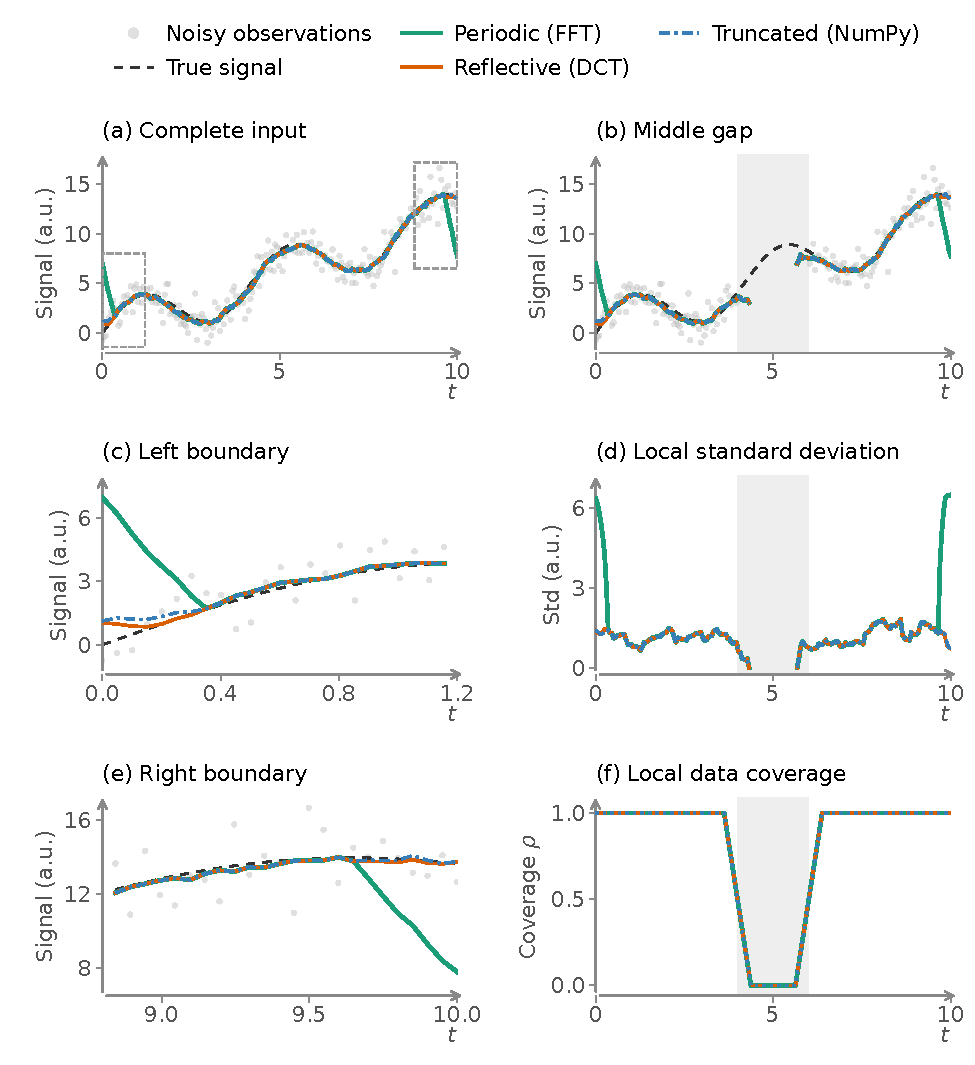
\includegraphics[width=\linewidth]{figures/round1/1d_boundary_comparison/pdf/boxcar_boundary_comparison.pdf}
	\caption{Width-15 boxcar boundary comparison ($N=200$, $r=0$, master seed 20261027): (a) complete observations and means; (c,e) endpoint zooms; (b) the same realization with a middle gap at $[80,120)$; (d) its population standard deviation; (f) its local data coverage. Gray points are observations; dashed black is the clean signal. Green/orange curves use periodic FFT/reflective DCT; blue dash-dot curves use truncated NumPy windows, clipped to the domain and renormalized over finite observations. The treatments agree to floating-point accuracy in full interior windows, subject to the near-zero standard-deviation qualification in the text. Gray shading marks missing inputs; curve breaks mark 26 undefined moments. Coverage uses each treatment's available weights; the three curves coincide here, with different line styles in (f). Moments require finite raw $d>10^{-3}$, without additive normalization or completion/restoration; 14 of 40 missing inputs have defined moments. Standard deviation is not uncertainty in the mean.}
	\label{fig:boxcar_missingness}
\end{figure}

\FloatBarrier
\subsection{Two-dimensional radar sweep}
\label{sec:radar_application}

For the real-data test, we use a COW C-band radar reflectivity sweep (the \texttt{DBZHC} field) collected during WINTRE-MIX on 23 February 2022. Its $720\times1180$ azimuth--range grid has a fixed elevation of $2^\circ$, nominal azimuth spacing of $0.5^\circ$, first gate center at 95~m, and nominal gate spacing of 74.9~m. The rays cover a complete circle without a repeated endpoint. Of the 849,600 grid cells, 508,956 contain finite observations; the remaining 40\% are missing. The mask therefore describes data availability.

We use Gaussian width settings $W=5$ and 15, with periodic boundaries in azimuth and reflective boundaries in range. The range width is $W$ gates, while the azimuth width is $W/[(j+1)\Delta_\phi]$ bins at range-gate index $j=0,1,\ldots$, where $\Delta_\phi$ is the azimuth spacing in radians. This index-based rule does not represent a fixed physical distance and has no special first-gate treatment. Azimuth filtering precedes range filtering for the moment inputs and the mask, with normalization after both stages. Moments are calculated from the dBZ field without conversion to linear reflectivity.

At the first gate, the azimuth widths are 573 and 1719 bins for $W=5$ and 15, respectively. For $W=15$, the width exceeds the 720-ray sweep at the first two gates. Each width sets the Gaussian bandwidth in Eq.~\ref{eq:tf_gaussian}, without rounding the width or imposing a sweep-length cap. The kernel radius is $\lceil4\sigma_{g,a}\rceil$, and circular filtering accumulates repeated contributions onto the same 720 rays rather than treating them as additional independent observations.

We compare the spectral calculation with standard spatial convolution using the same range-dependent polar Gaussian filter. In this experiment, standard spatial convolution denotes an explicit implementation in which each axis stage visits every azimuth--range output cell in nested Python loops and evaluates its Gaussian neighbourhood using a NumPy dot product. The two stages retain the prescribed boundaries and angular-first order. Both implementations are also checked against an independent spatial reference, which uses samples verified against Astropy \texttt{Gaussian1DKernel} and calculates centered-residual variances without convolution routines, spectral transforms, or raw-moment subtraction. We assess every cell of the full sweep and separately report the 95,760 cells within 10~km of the radar, where the azimuth widths are largest.

% Source: experiments/results/round1/v2.0.0/2d_radar_gaussian_double_loop/
% release-v2-20261111/{agreement_summary,spectral_loop_comparison}.csv.
% Default floor 1e-3; direct discrete_spectral vs explicit_spatial_double_loop.
% Variance discrepancies use the raw moment difference before clamping.

\begin{table}[htbp]
	\centering
	\caption{Spectral Gaussian radar statistics against standard spatial convolution, implemented with explicit Python double loops, on the original missing-data pattern at $\epsilon=10^{-3}$. Compared moment counts $n_c$ are out of 849,600 cells for the full sweep and 95,760 near the radar (range $\leq10$~km). Entries are maximum absolute differences between the two calculations, in dBZ for mean and dBZ$^2$ for variance. Variance is checked before clamping; the independent centered-residual check is separate.}
	\label{tab:radar_statistics}
	\small
	\setlength{\tabcolsep}{4pt}
	\begin{tabular}{@{}llrrr@{}}
		\toprule
		$W$ & Region & $n_c$ & Mean difference & Variance difference \\
		\midrule
		5 & Full sweep & 574592 & $2.12\times10^{-11}$ & $8.69\times10^{-10}$ \\
		5 & Near radar & 77889 & $1.78\times10^{-11}$ & $7.88\times10^{-10}$ \\
		15 & Full sweep & 640682 & $1.76\times10^{-11}$ & $4.39\times10^{-10}$ \\
		15 & Near radar & 90140 & $3.18\times10^{-12}$ & $1.81\times10^{-10}$ \\
		\bottomrule
	\end{tabular}
\end{table}

The spectral calculation agrees closely with standard spatial convolution (Table~\ref{tab:radar_statistics}), with identical defined-output masks. Across both widths, their maximum mean and raw-variance discrepancies are $2.12\times10^{-11}$~dBZ and $8.69\times10^{-10}$~dBZ$^2$. Both also agree with the independent centered-residual reference. Defined moments cover 67.63\% and 75.41\% of the original sweep for $W=5$ and 15, respectively. These counts include estimates at missing input locations, but do not establish recovery of unknown reflectivity values.

The spectral raw-variance minima are $-7.22\times10^{-11}$ and $-1.81\times10^{-10}$~dBZ$^2$ for $W=5$ and 15, consistent with floating-point error against the centered-residual reference. The largest standard-deviation difference is $1.84\times10^{-5}$~dBZ near zero variance, where taking the square root amplifies small moment differences. Raw variance is checked before clamping with absolute tolerance $2\times10^{-6}$~dBZ$^2$ and relative tolerance $2\times10^{-9}$. Where the reference variance is at most this absolute tolerance, the standard-deviation check uses the square root of the variance-error bound. The comparison uses the original missing-data pattern at one denominator floor; controlled-removal and floor-sensitivity tests of this Gaussian kernel were not performed.

Figure~\ref{fig:radar_statistics} shows the original sweep and its mean, reported standard deviation, and local data coverage for $W=15$. The enlarged views show a $20\times20$~km square after filtering the full sweep. Its corners extend beyond the circular near-radar region used in Table~\ref{tab:radar_statistics}.

\begin{figure}[pos=p,belowcap=0pt]
	\centering
	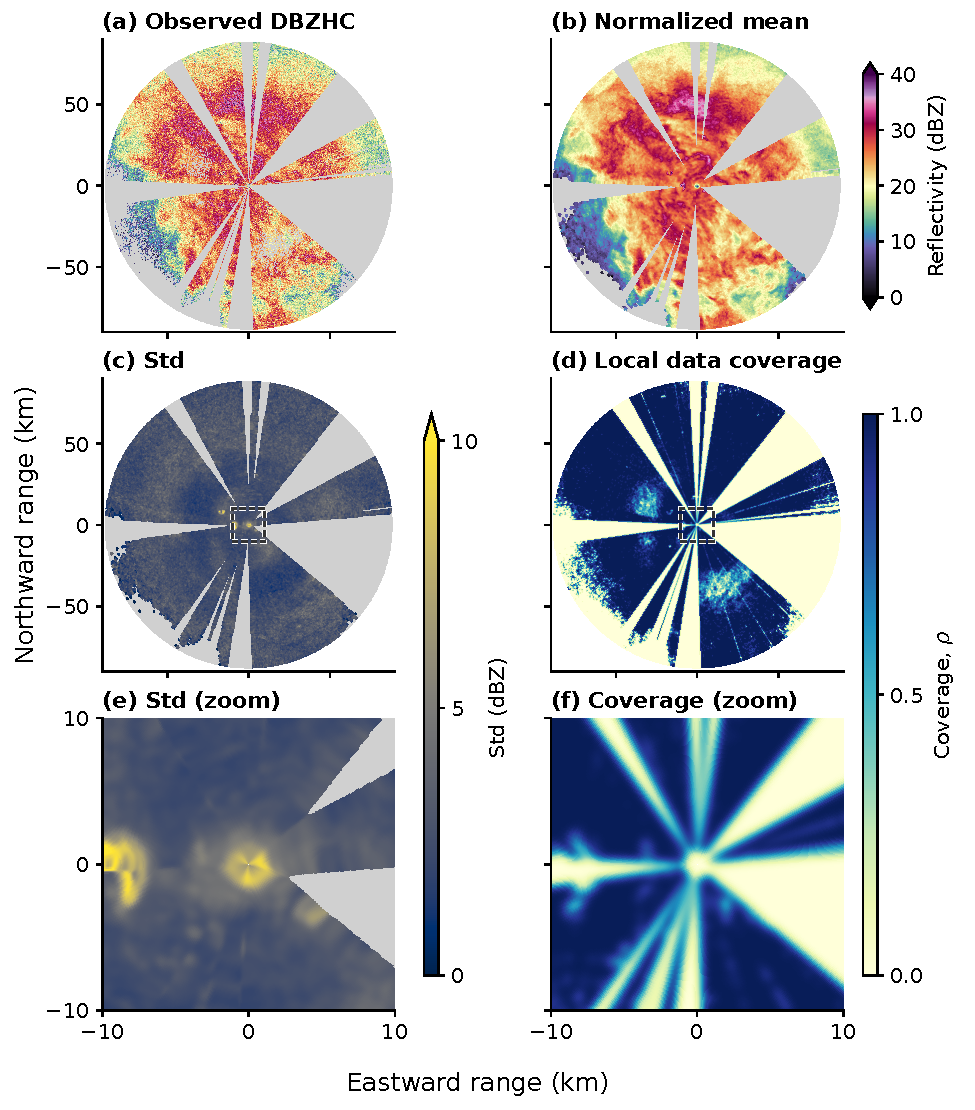
\includegraphics[width=\linewidth]{figures/round1/2d_radar_discrete_gaussian/pdf/radar_gaussian_statistics.pdf}
	\caption{COW sweep 12 with Gaussian $W=15$ (legacy index units): (a) observations; (b) normalized mean; (c,e) standard deviation; (d,f) local data coverage. Panels (e--f) enlarge $x,y\in[-10,10]$~km (dashed squares in c--d) after full-sweep filtering. Maps use native azimuths and slant ranges, not surface distances. Moments require finite raw $d>10^{-3}$; no completion or input-mask restoration is used. Gray marks missing observations in (a) and undefined estimates in (b,c,e). Panels (a--b) share cmweather ChaseSpectral over $0$--$40$~dBZ; standard-deviation panels share $0$--$10$~dBZ, with colorbar extensions for out-of-range values. Coverage $\rho$ describes weighted data availability, not measurement quality or uncertainty.}
	\label{fig:radar_statistics}
\end{figure}

\FloatBarrier
\subsection{Three-dimensional synthetic wind field}

The final example is a synthetic three-dimensional wind field. The synthetic wind field combines a height-modulated tangential circulation, a localized vertical core, and weak background variations on a baseline $(z,y,x)$ grid of $18\times96\times96$ cells. Each signed component $u$, $v$, and $w$ receives independent normal perturbations of standard deviation 0.14 in arbitrary normalized velocity units. Vector anomalies occur with probability 0.003, with isotropic directions and amplitudes uniform on $[1.25,2.25]$ in the same units. Separate NumPy random streams use seeds 4101 for noise, 4102 for anomalies, and 4103 for missingness, giving one realization at each grid shape. Equal-shaped cases reuse these realizations, and the random 20\% and 50\% removal masks are nested. The common validity mask is the intersection of finite $u$, $v$, and $w$; missingness is independent of anomaly injection.

We calculate each wind component separately. We calculate separate component moments over the spatial axes using the reflective odd boxcar $(3,7,7)$, never smoothing across a component index or replacing the components by wind speed. NumPy symmetric-window reductions provide the independent reference for a prepared DCT implementation, the untimed released statistics API, SciPy uniform filtering, and Astropy direct and FFT convolutions. Astropy uses explicit symmetric padding and cropping to match reflection; every method uses identical incomplete inputs and direct-ratio rules. Table~\ref{tab:wind_component_agreement} gives componentwise discrepancies for the baseline 20\% case, whose actual missing fraction is 20.1829\%. All 165,888 cells per component have defined moments, including the 33,481 missing-input locations.

% Source: experiments/results/round1/v2.0.0/3d_wind_boxcar/release-v2-20261111/.
% comparison.csv: baseline20, whole_domain; maxima over all five methods
% relative to numpy_windows, retaining the untimed released-API validation.
% All cases/regions: 1,920 pass / 390 no_comparable / 0 fail (2,310 rows).

\begin{table}[pos=hbp]
	\centering
	\caption{Maximum absolute componentwise discrepancies against NumPy for the baseline 3D wind case with requested 20\% missingness, pooled over the five checked implementations. Each moment uses all 165,888 cells. Mean and standard-deviation differences are in normalized velocity units, variance differences in squared units, and equivalent-count differences in cells.}
	\label{tab:wind_component_agreement}
	\small
	\begin{tabular}{@{}lrrrr@{}}
		\toprule
		Component & $\max|\Delta\mu|$ & $\max|\Delta\sigma^2|$ & $\max|\Delta\sigma|$ & $\max|\Delta N_{\mathrm{eq}}|$ \\
		\midrule
		$u$ & $3.11\times10^{-15}$ & $6.22\times10^{-15}$ & $2.10\times10^{-14}$ & $1.99\times10^{-13}$ \\
		$v$ & $2.89\times10^{-15}$ & $7.11\times10^{-15}$ & $2.17\times10^{-14}$ & $1.99\times10^{-13}$ \\
		$w$ & $4.44\times10^{-16}$ & $2.64\times10^{-16}$ & $4.72\times10^{-16}$ & $1.99\times10^{-13}$ \\
		\bottomrule
	\end{tabular}
\end{table}

Figure~\ref{fig:wind_statistics} displays observed and componentwise local-mean wind in three dimensions; classification diagnostics are in Section~\ref{sec:discussion}. Only one component's standard deviation is displayed for clarity; all three components are calculated and checked separately.

\begin{figure}[pos=p,belowcap=0pt]
	\centering
	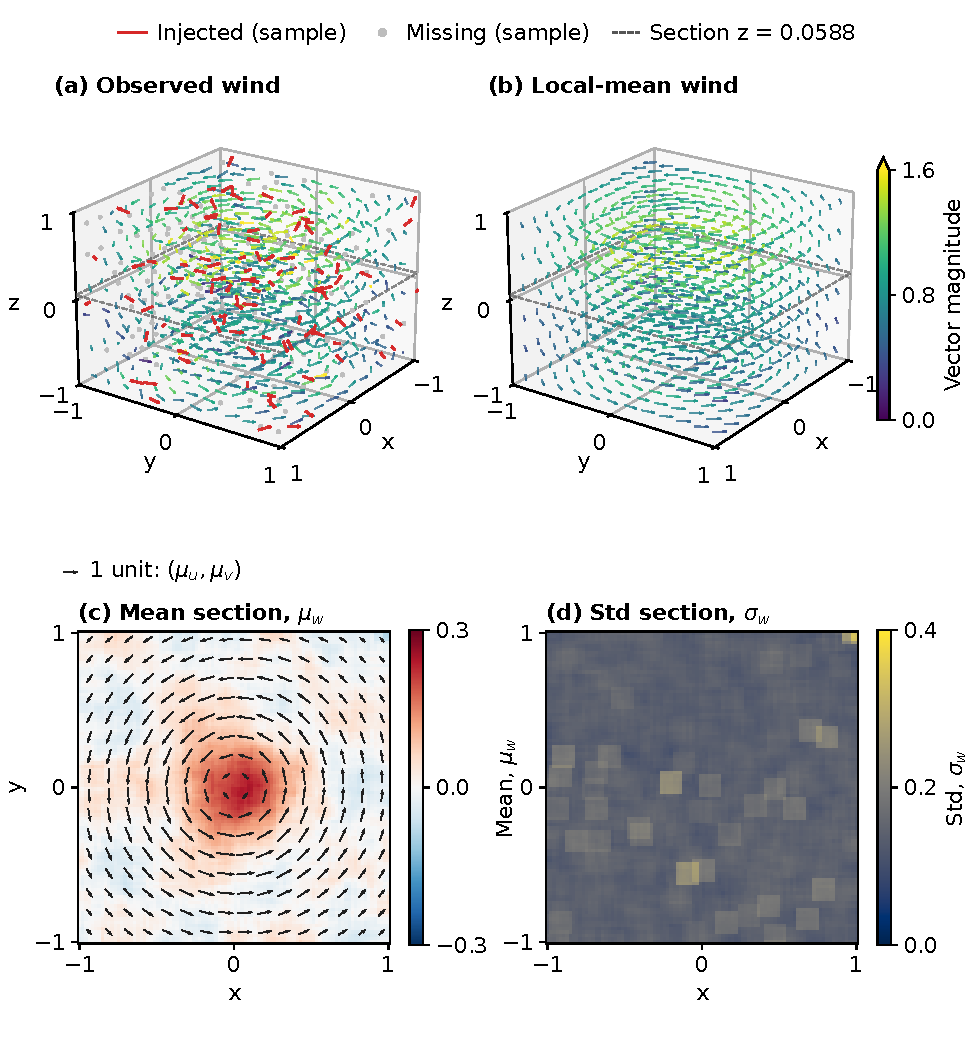
\includegraphics[width=\linewidth]{figures/round1/3d_wind_boxcar/pdf/wind_component_statistics.pdf}
	\caption{Observed wind and local statistics for the $18\times96\times96$ baseline case with 20.1829\% missingness and full-volume reflective $(3,7,7)$ boxcars. Panels (a--b) use the same display lattice, with $(z,y,x)$ strides $(3,8,8)$; gray points in (a) mark sampled missing inputs. The 3D arrows have fixed display length, and viridis colours encode the observed vector magnitude or the magnitude of the componentwise mean vector, not mean wind speed. Red arrows identify 100 sampled observed injections, not detected anomalies. Dashed outlines mark zero-based plane 9 ($z=0.0588$), shown in (c--d) as $\mu_w$ and population standard deviation $\sigma_w$. In (c), $(\mu_u,\mu_v)$ arrows use stride 6 and the displayed length key. Sampling is for display only; coordinates are normalized and velocity units arbitrary. All moments satisfy finite raw $d>10^{-3}$ without completion or restoration. Estimates at missing-input locations are not recovered observations; standard deviation describes local variation, not uncertainty in the mean.}
	\label{fig:wind_statistics}
\end{figure}

We also test a few variations of grid and window. Additional checks use $18\times48\times48$ and $24\times128\times128$ grids, narrower $(3,3,3)$ and broader $(5,15,15)$ windows, a missing $z$ plane, a central missing block, and all-missing and single-observation controls. Over all 11 cases, maximum discrepancies are $2.73\times10^{-14}$ for mean, $4.06\times10^{-14}$ for variance, and $2.08\times10^{-11}$ cells for $N_{\mathrm{eq}}$, with matching defined-output masks. The largest standard-deviation discrepancy, $1.12\times10^{-8}$, occurs in the single-observation control near zero variance; its variance discrepancy is at most $1.39\times10^{-16}$. Table~\ref{tab:wind_coverage_flags} distinguishes accepted moment coverage from observed inputs: the missing block leaves 108 undefined cells, while only 147 of 720 cells have defined moments in the single-observation control. All-missing moments remain undefined and both coverage and equivalent count are zero.

Finally we show one descriptive use of the moments. For a descriptive application, component $c\in\{u,v,w\}$ is flagged when $|x_c-\mu_c|>3\sigma_c$, only at observed cells with $\rho\geq0.35$, finite mean and standard deviation, and $\sigma_c>10^{-8}$ normalized velocity units. Flags remain separate among components; missing observations cannot be flagged. The additional eligibility gate is distinct from acceptance of a moment ratio: for example, all moments are defined in the 50\% case, but 66 of its 82,707 observed cells are ineligible for scoring. Table~\ref{tab:wind_coverage_flags} reports fixed-criterion counts, not correct-detection counts or an optimized threshold. Each candidate is included in its own moments and can shift the local mean and inflate dispersion, reducing its score. This illustration neither mitigates that self-influence nor establishes detector accuracy through threshold tuning or independent evaluation.

% Same 3D run: comparison.csv, dct_shared_moments, whole_domain, mean,
% n_compared (identical for all components/moments/methods); application_counts.csv
% gives n_observed, n_eligible, n_flagged. No detection-performance aggregation.
\begin{table}[htbp]
	\centering
	\caption{3D moment coverage and descriptive flags for selected missingness cases, using $(3,7,7)$ boxcars. Random percentages denote requested removal probabilities. Counts refer to spatial cells per component, not the sum over components. Compared counts are jointly defined moment outputs; defined-output masks match across methods. Observed and eligible counts are common to $u,v,w$. The final column lists separate flag counts in that order.}
	\label{tab:wind_coverage_flags}
	\small
	\setlength{\tabcolsep}{4pt}
	\begin{tabular}{@{}llrrrl@{}}
		\toprule
		Input mask & Grid $(z,y,x)$ & Observed & Compared & Eligible & Flags $(u,v,w)$ \\
		\midrule
		Complete & $18\times96\times96$ & 165888 & 165888 & 165888 & $(488,469,651)$ \\
		Random 20\% & $18\times96\times96$ & 132407 & 165888 & 132407 & $(378,357,508)$ \\
		Random 50\% & $18\times96\times96$ & 82707 & 165888 & 82641 & $(240,241,306)$ \\
		Missing plane & $18\times48\times48$ & 39168 & 41472 & 39168 & $(104,93,150)$ \\
		Missing block & $10\times24\times24$ & 5040 & 5652 & 5040 & $(12,10,25)$ \\
		Single observation & $5\times12\times12$ & 1 & 147 & 0 & $(0,0,0)$ \\
		All missing & $5\times12\times12$ & 0 & 0 & 0 & $(0,0,0)$ \\
		\bottomrule
	\end{tabular}
\end{table}

%% ========================================================================
\FloatBarrier
\section{Computational performance}
\label{sec:performance}

\subsection{Three-dimensional benchmark setup}
\label{sec:benchmark_setup}

We ask what the matched workload costs on this machine. The 3D comparison measures the same componentwise statistics with different filtering implementations. Every calculation applies seven full-volume filters: one to the common validity mask, then one to each of $u,v,w$ and its square. Each component mean is reused in its clamped population variance, whose square root gives standard deviation; the mask response and equivalent-count array are shared across components. All methods use identical inputs, odd boxcars, half-sample reflection, and the strict acceptance rule of finite $d>10^{-3}$. Completion and input-NaN restoration are disabled; these are not costs of the default gap-completion procedure.

Every method prepares its filter once per timed calculation and reuses it for the seven fields. The experiment-local DCT implementation constructs axis responses using the released v2.0.0 \texttt{get\_dct\_transfer\_function}, then applies them within each N-D DCT/multiply/inverse-DCT sequence. The released statistics API is checked numerically in a separate untimed comparison. NumPy reduces symmetric sliding-window views one output $z$ plane at a time, without materializing all windows. Astropy direct and FFT convolution reuse one dense spatial kernel and explicitly pad and crop each filtered field to match reflection. Astropy FFT's internal per-call padding and kernel transforms remain included; no cached kernel FFT is assumed.

We run the measurements on one machine with one thread. Measurements ran sequentially on an Apple M4 Pro with 24~GiB RAM, using x86\_64 Python 3.11.13 under Rosetta~2, not native ARM Python, with NumPy 2.4.4, SciPy 1.17.1, and Astropy 8.0.2. Numerical-library thread limits were requested as one. Each 3D method--case pair has three fresh-worker repetitions, with method order rotated and no filter warm-up. Workers preload the same libraries and use matching input hashes.

We time each calculation from the resident inputs to the returned outputs. Wall-clock timing starts with resident inputs and includes mask construction, zero replacement, padding, filter preparation, seven filters, normalization, variance, square roots, and output allocation. Input generation, imports, I/O, plotting, and anomaly flagging are excluded.

\subsection{Three-dimensional runtime and memory}
\label{sec:benchmark_memory}

The 3D table shows a trade-off, not a universal ranking. Table~\ref{tab:performance_time} compares selected implementations, not all spatial algorithms. The SciPy 1.17.1 \href{https://github.com/scipy/scipy/blob/v1.17.1/scipy/ndimage/_filters.py\#L1550-L1618}{\texttt{uniform\_filter}} calculation uses the same boxcar estimator, mask normalization, seven filters, and outputs, and has a lower median time than prepared DCT in all eight cases. For the $18\times96\times96$ grid with a $(3,7,7)$ window and 20.18\% missingness, its median is 0.0162~s versus 0.0297~s for DCT. Its separable one-dimensional running sums in \href{https://github.com/scipy/scipy/blob/v1.17.1/scipy/ndimage/src/ni_filters.c\#L311-L374}{\texttt{NI\_UniformFilter1D}} give approximately $\mathcal{O}(N)$ cost for $N$ cells at fixed dimensionality and ordinary window sizes, rather than the $\mathcal{O}(NK)$ cost of generic direct convolution with $K$ window cells. These timings therefore do not establish superiority over optimized spatial boxcar filtering.

% Source: experiments/results/round1/v2.0.0/3d_wind_boxcar/
% release-v2-20261111/{benchmark_runs,benchmark_summary,settings}.csv.
% Times are medians recomputed from the three successful raw repetitions;
% memory entries below are their maximum peak_ram_mib, not peak minus baseline.
% All five methods and all eight cases remain in the accompanying CSV files.
\begin{table}[pos=hbp]
	\centering
	\caption{Median elapsed time (s) over three fresh-worker repetitions of the matched seven-filter 3D statistics calculation, including preparation. Grid and window dimensions are ordered $(z,y,x)$; widths are in grid cells and do not preserve a physical footprint across resolutions. Missingness is the actual percentage. Missing cells are randomly placed except in the missing-plane row (${}^{\mathrm{p}}$). DCT is the experiment-local prepared implementation; direct and FFT columns are Astropy. SciPy computes the same workload with lower medians than DCT in all eight cases (0.0162~s versus 0.0297~s for the 20.18\%-missing $(3,7,7)$ baseline).}
	\label{tab:performance_time}
	\setlength{\tabcolsep}{4pt}
	\begin{tabular*}{\linewidth}{@{\extracolsep{\fill}}lrrrrrr@{}}
		\toprule
		Grid & Window & Missing (\%) & DCT & NumPy & \multicolumn{2}{c}{Astropy} \\
		\cmidrule(l){6-7}
		 & & & & & Direct & FFT \\
		\midrule
		$18\times48\times48$ & $(3,7,7)$ & 20.47 & 0.0069 & 0.0940 & 0.0293 & 0.0290 \\
		$18\times96\times96$ & $(3,7,7)$ & 0.00 & 0.0320 & 0.3693 & 0.1049 & 0.1071 \\
		$18\times96\times96$ & $(3,7,7)$ & 20.18 & 0.0297 & 0.3725 & 0.1042 & 0.1015 \\
		$18\times96\times96$ & $(3,7,7)$ & 50.14 & 0.0309 & 0.3777 & 0.1064 & 0.1082 \\
		$24\times128\times128$ & $(3,7,7)$ & 20.06 & 0.0937 & 0.8842 & 0.2402 & 0.2378 \\
		$18\times96\times96$ & $(3,3,3)$ & 20.18 & 0.0315 & 0.1350 & 0.0315 & 0.1050 \\
		$18\times96\times96$ & $(5,15,15)$ & 20.18 & 0.0321 & 1.4970 & 1.2891 & 0.1740 \\
		$18\times48\times48$ & $(3,7,7)$ & $5.56^{\mathrm{p}}$ & 0.0074 & 0.0942 & 0.0298 & 0.0324 \\
		\bottomrule
	\end{tabular*}
\end{table}

Window width changes the relative costs. For the narrow $(3,3,3)$ window, Astropy direct and DCT have nearly equal median times (both 0.0315~s after rounding), with overlapping interquartile ranges. Astropy direct's median increases to 1.2891~s for $(5,15,15)$, whereas DCT takes 0.0321~s. NumPy window reductions also become more expensive across these wider-window cases. DCT medians vary little across these window choices, but SciPy retains lower medians, taking 0.0142 and 0.0141~s for the narrow and broad cases. Missing data do not reduce the number or extent of filtering passes. The size and missingness comparisons in Table~\ref{tab:performance_time} describe these implementations on this machine; three repetitions and a few sizes do not establish an asymptotic law or a reliable crossover.

Memory shows no uniform ranking. Peak process resident set size (RSS) is sampled at 1-ms intervals and supplemented by the native lifetime high-water mark only when the timed call exceeds its previous value. Table~\ref{tab:performance_ram} reports the maximum peak over the three repetitions, in MiB ($2^{20}$ bytes). RSS includes native arrays, resident inputs, and the matched preloaded libraries, not just filter allocations. Before-call RSS is recorded separately; subtracting it does not give an exact allocation count. If no new lifetime peak is reached, shorter-lived peaks can be missed between samples.

SciPy's maximum RSS is 154.4~MiB for the 20.18\%-missing $(3,7,7)$ baseline and 201.4~MiB for the larger volume, compared with 135.0 and 209.9~MiB for DCT, respectively; there is no uniform memory ranking between them. Individual repetitions, quartiles, before-call RSS, and all SciPy measurements accompany this revision.

\begin{table}[pos=htbp]
	\centering
	\caption{Maximum measured total process RSS (MiB) for the same configurations and three repetitions as Table~\ref{tab:performance_time}. These peaks include common inputs and libraries and are not algorithm-only memory allocations. The superscript p denotes the missing-plane mask.}
	\label{tab:performance_ram}
	\setlength{\tabcolsep}{4pt}
	\begin{tabular*}{\linewidth}{@{\extracolsep{\fill}}lrrrrrr@{}}
		\toprule
		Grid & Window & Missing (\%) & DCT & NumPy & \multicolumn{2}{c}{Astropy} \\
		\cmidrule(l){6-7}
		 & & & & & Direct & FFT \\
		\midrule
		$18\times48\times48$ & $(3,7,7)$ & 20.47 & 113.6 & 112.7 & 119.2 & 139.4 \\
		$18\times96\times96$ & $(3,7,7)$ & 0.00 & 145.2 & 153.5 & 174.0 & 233.6 \\
		$18\times96\times96$ & $(3,7,7)$ & 20.18 & 135.0 & 153.0 & 174.0 & 273.0 \\
		$18\times96\times96$ & $(3,7,7)$ & 50.14 & 140.5 & 154.9 & 183.9 & 289.5 \\
		$24\times128\times128$ & $(3,7,7)$ & 20.06 & 209.9 & 218.9 & 268.4 & 316.6 \\
		$18\times96\times96$ & $(3,3,3)$ & 20.18 & 161.6 & 152.2 & 169.6 & 290.2 \\
		$18\times96\times96$ & $(5,15,15)$ & 20.18 & 145.6 & 160.9 & 187.1 & 361.8 \\
		$18\times48\times48$ & $(3,7,7)$ & $5.56^{\mathrm{p}}$ & 114.2 & 109.1 & 121.7 & 149.1 \\
		\bottomrule
	\end{tabular*}
\end{table}

\FloatBarrier
\subsection{Radar runtime and memory}
\label{sec:radar_performance}

The radar benchmark compares spectral filtering with standard spatial convolution as defined in Section~\ref{sec:radar_application}, using the original $720\times1180$ incomplete sweep at $W=5,15$. Spectral filtering constructs the Gaussian responses and applies RFFT in azimuth and DCT-II in range. Standard spatial convolution instead uses explicit Python double loops over the output azimuth and range indices in each axis stage, with NumPy dot products for the one-dimensional Gaussian sums. Both implementations calculate the same ordered polar filter.

Each implementation prepares once and applies three complete filters to the finite mask, zero-filled observations, and their squares, with normalization only after both axis stages. Common code calculates mean, variance, standard deviation, coverage, and equivalent count, using finite raw $d>10^{-3}$ without completion or restoration. Five fresh-worker repetitions per width use matching imports, rotated method order, requested one-thread limits, and no warm-up on the machine described in Section~\ref{sec:benchmark_setup}. Timings include masking, kernel and response preparation, boundary padding, filtering, normalization, and allocation; input reading and numerical verification are excluded. Workers verify source, input, all nine output arrays, and preparation/filter counts; the loop implementation also records its actual cell updates in each stage. RSS follows Section~\ref{sec:benchmark_memory}. These are prepared shared-filter calculations, not separate released statistics-API calls.

% Source: experiments/results/round1/v2.0.0/2d_radar_gaussian_double_loop/
% release-v2-20261111/{benchmark_runs,benchmark_summary,benchmark_phases,settings}.csv.
\begin{table}[pos=hbp]
	\centering
	\caption{Radar runtime and memory for five fresh-worker repetitions, including preparation, boundary padding, and three complete filters. Spectral filtering and standard spatial convolution (explicit Python double loops) use the same polar Gaussian filter. Times are medians in seconds; RSS is the maximum total process peak in MiB.}
	\label{tab:radar_performance}
	\setlength{\tabcolsep}{3pt}
	\begin{tabular*}{\linewidth}{@{\extracolsep{\fill}}lrrrr@{}}
		\toprule
		$W$ & \multicolumn{2}{c}{Time (s)} & \multicolumn{2}{c}{Peak RSS (MiB)} \\
		\cmidrule(lr){2-3}\cmidrule(l){4-5}
		 & Spectral & Standard & Spectral & Standard \\
		\midrule
		5 & 0.0798 & 3.8404 & 248.9 & 252.4 \\
		15 & 0.0841 & 3.7916 & 235.2 & 250.1 \\
		\bottomrule
	\end{tabular*}
\end{table}

Table~\ref{tab:radar_performance} gives spectral speedups of 48.1 and 45.1 over standard spatial convolution at $W=5$ and 15, respectively, calculated from the unrounded medians. These ratios compare the spectral implementation with the stated Python cell loops and NumPy neighbourhood sums, not a general advantage over optimized spatial filtering. Median preparation costs are 22.70/23.22~ms for spectral filtering and 6.34/6.46~ms for standard spatial convolution, ordered by $W=5/15$. These costs are already included in the totals; per-filter boundary padding is included separately within total runtime. Five repetitions on one sweep and two widths do not establish a general ranking or crossover.

\FloatBarrier
\subsection{Additional mean-only benchmarks}

% Source: experiments/results/round1/3d_large_boxcar_mean/
% quick-large-mean-1gib-20261027/{benchmark_runs,benchmark_summary,settings,comparison}.csv.
A separate exploratory check retained from v1.0.0 uses one scalar $512^3$ \texttt{float64} input (1~GiB), with 19.9983\% missing values. SciPy uniform and prepared DCT filtering use reflective boxcars and the same direct-ratio rule, overwriting their input and mask buffers. Timing includes mask construction, zero replacement, preparation, two filters, and mean normalization, not the full three-component statistics. From two fresh-worker repetitions per method and width, median SciPy times are 13.980 and 13.853~s for $3^3$ and $31^3$ boxcars, respectively; DCT takes 15.583 and 15.510~s, about 12\% longer. Maximum recorded total RSS is approximately 2.34~GiB, using before/after RSS and any newly exceeded lifetime high-water mark rather than interval sampling.

Small-array checks cover every output cell, but the large outputs are compared only at 2,173 fixed boundary and random sample locations, with maximum mean discrepancy $2.50\times10^{-15}$. Native swap counters do not increase during timing, although the host has pre-existing memory pressure. A separate headroom check found insufficient memory for the guarded 2-GiB case, so that input was not allocated. This mean-only experiment examines window-width sensitivity at one input size; the similar-order runtimes do not establish dataset-size scaling or a crossover.

The retained analytical-Gaussian radar comparisons and mean-only timings are documented separately in the experiment archive. They are not measurements of the Gaussian convolution in Table~\ref{tab:radar_performance}. The 1D example has no timing study.

%% ========================================================================
\section{Discussion}
\label{sec:discussion}

Using one complete filter for all moment inputs and the original mask keeps the statistics and availability diagnostics consistent with the same geometry and boundary assumptions. We integrate established spectral filtering \citep{Oppenheim1999,Martucci1994} and normalized convolution \citep{Knutsson1993,Westin1994,Pham2006} with the range-dependent, two-dimensional angle--range construction described by \citet{Valdivia2026RadarDCT}. The contribution is this integration, not new filter or normalization theory or exclusive per-axis control.

Explicit geometry broadens the configurations that can be specified, but its widths remain coordinate-line scales on regular tensor grids. Geometry-dependent stages follow a prescribed order, so they should not be interpreted as isotropic, geodesic, or cell-volume-weighted averaging. The real-data example tests only a 2D polar sweep with legacy index-unit widths, not fixed physical-distance windows or N-D observational configurations. The 3D wind example is Cartesian and does not extend that polar evidence.

Agreement with matched references isolates numerical consistency from estimation quality; it does not establish superiority over boundary-matched alternatives. The radar comparison uses the original incomplete input without testing recovery of unknown values. The 1D truth errors characterize one known synthetic signal on its defined-output domain, not general gap-recovery accuracy; naturally missing radar values remain unknown. Because all comparisons and timings disable completion, the accuracy and cost of the default fallback remain unassessed. No same-data comparison with the prior interpolation-first workflow was performed.

For nonnegative, constant-preserving spatial weights, local data coverage describes weighted availability, and direct ratios with an accepted positive denominator give a bounded mean and a nonnegative weighted population variance in exact arithmetic. The equivalent data count expresses coverage on a nominal-width scale, not generally as a count of distinct observations or a statistical effective sample size. The moments are descriptive rather than unconditionally unbiased estimates; neither coverage diagnostic by itself measures uncertainty.

The denominator floor is a numerical acceptance choice, not a statistical reliability threshold. The radar Gaussian comparison checks one fixed floor and its original missing-data pattern; it does not establish sensitivity to that choice or evaluate additional controlled removal. The agreement with centered-residual variances separates floating-point moment cancellation from differences in the estimator, but does not quantify uncertainty or validate default completion.

The componentwise wind flags illustrate one use of local moments, not a validated anomaly detector. In the baseline 20\% case, 406 of the 521 vector-injection locations remain observed and eligible; the 115 missing injections are excluded from classification. Comparing each component's flags with the vector-injection labels gives true-positive, false-positive, and false-negative counts of $(286,92,120)$ for $u$, $(270,87,136)$ for $v$, and $(290,218,116)$ for $w$. These are separate component diagnostics, not a combined vector detector; injections need not strongly affect every component. Each candidate contributes to its own mean and dispersion and can reduce its own score, but these counts do not isolate that effect. The fixed $k=3$ criterion is an illustrative choice, not an optimal or independently calibrated threshold.

One possible extension is to exclude or downweight suspect observations and recompute local moments before applying the screening bands $\mu_c\pm3\sigma_c$. For exclusion, the revised mask must enter both moment numerators and normalization; rejected observations are not valid zeros, and the original availability mask remains distinct from later quality-control exclusions. \citet{Garcia2010} uses iterative residual-based reweighting in a DCT-based penalized smoother, a different estimator from the normalized boxcar moments used here. For instrument data, \citet{Vitale2021} reviews iterative mean/standard-deviation despiking and robust location and scale alternatives for eddy covariance measurements, evaluating classifications and recovered variance. These approaches may reduce contamination, but missed anomalies can remain influential, genuine flow structures can be rejected, and selective removal can underestimate variability. No iterative rejection, robust reweighting, or independent detector evaluation was performed here; improved screening or variance estimation requires separate validation, and the screening bands are not confidence intervals.

The runtime differences reflect how each implementation evaluates the matched filter. Spectral filtering replaces repeated neighbourhood sums with fast transforms and multiplication by prepared responses; after preparation, wider kernels on a fixed grid do not increase the transform dimensions. For polar filtering, range-dependent angular responses are applied across range gates through array operations rather than output-cell loops. Reflective DCT filtering acts on the original grid, whereas the benchmarked Astropy FFT calculation includes explicit reflection padding and per-call kernel transforms. These differences do not imply a lower asymptotic cost than FFT convolution. The spatial radar baseline also incurs Python-loop and per-neighbourhood call overhead. The measurements do not separate the effects of transform evaluation, boundary handling, and Python overhead. Each method prepares its spatial kernel or spectral response once and uses the same three- or seven-filter workload, so the spectral method does not perform fewer filtering passes. SciPy's specialized running-sum boxcar is faster in every measured 3D full-statistics case, while Astropy direct convolution and DCT have nearly equal medians for the narrowest window. The timings therefore concern the stated prepared implementations, not a general advantage over optimized spatial filtering or the cost of separate released statistics-API calls.

The similar-order runtimes in the separate 1-GiB mean check should not be extrapolated to full-statistics scaling or a crossover: it uses two in-place filters, two repetitions, one input size, and sampled output comparisons. All benchmarks ran under Rosetta~2, whose effect on relative performance was not measured. Process RSS also includes inputs and libraries, so the reported peaks guide resource planning rather than quantify filter allocations alone.

For radar, the calculations operate on dBZ, so their dispersion outputs do not directly quantify linear-reflectivity variability or measurement-noise uncertainty. The finite-value mask records availability rather than measurement quality, and upstream QC remains unverified. Practical use therefore requires application-specific validity, width, and acceptance choices. Neither finite output nor high local data coverage supplies automatic quality assurance, and these experiments establish no universal coverage cutoff.

%% ========================================================================
\section{Conclusion}
\label{sec:conclusion}

Building on established spectral filters and normalized convolution, this work unifies masked local mean, variance, standard deviation, and data-availability diagnostics through the same complete operator. It combines independent per-axis kernel and boundary choices with reflective Cartesian filtering and explicit geometry on regular N-D polar grids. Agreement with weight- and boundary-matched references is demonstrated for 1D discrete boxcars with missing observations, Gaussian statistics on one real 2D COW radar sweep, and componentwise 3D Cartesian wind boxcars with explicit missingness. Local data coverage $\rho$ and equivalent data count $N_{\mathrm{eq}}$ provide diagnostics of the filtered mask, not uncertainty estimates; $N_{\mathrm{eq}}$ is not generally an observation count or statistical effective sample size.

The matched runtime and process-RAM results show implementation-dependent trade-offs, not a universal ranking. SciPy's running-sum boxcar computes the same estimator faster than prepared DCT in every tested 3D full-statistics case, while Astropy direct convolution and DCT have nearly equal medians for the narrowest window. On the radar sweep, the spectral Gaussian calculation is approximately 45--48 times faster than standard spatial convolution implemented with explicit Python double loops. These timings describe the stated shared-filter implementations, not separate released statistics-API calls or an intrinsic advantage over optimized spatial filtering. Numerical agreement on the same incomplete input does not establish recovery of unknown values or statistical reliability. These direct-ratio tests do not assess default completion or provide observational validation of N-D polar processing.

%% ========================================================================
\section*{Acknowledgments}

This research was sponsored by the National Science Foundation grant AGS~2114011.

\noindent\textbf{Code availability section}

\begin{description}
\item[Name of the code/library] \texttt{dct-toolkit}, imported in Python as \texttt{dct\_toolkit}
\item[Contact] Jairo M.~Valdivia (\texttt{jairo.valdiviaprado@colorado.edu})
\item[Hardware requirements] Standard workstation (CPU). GPU is not required.
\item[Program language] Python $\ge$ 3.8
\item[Software required] NumPy $\ge$ 1.20; SciPy $\ge$ 1.8. These and Python $\ge$ 3.8 are the runtime requirements declared in the released v2.0.0 \href{https://github.com/JValdivia23/dct-toolkit/blob/7ff29e998dd1102d3fef2a84050402e86dc7ef67/pyproject.toml}{\texttt{pyproject.toml}}; the actual experiment environment is specified in Section~\ref{sec:validation}.
\item[Source codes] The toolkit is publicly available at \url{https://github.com/JValdivia23/dct-toolkit} under the \href{https://github.com/JValdivia23/dct-toolkit/blob/7ff29e998dd1102d3fef2a84050402e86dc7ef67/LICENSE}{MIT license} and on \href{https://pypi.org/project/dct-toolkit/2.0.0/}{PyPI}. This revision uses released v2.0.0, \href{https://github.com/JValdivia23/dct-toolkit/commit/7ff29e998dd1102d3fef2a84050402e86dc7ef67}{commit \texttt{7ff29e9}}. The matched four-sigma radar calculation remains in the accompanying experiment sources; it is distinct from the release's full Gaussian default.
\item[Documentation] The release includes a \href{https://github.com/JValdivia23/dct-toolkit/blob/7ff29e998dd1102d3fef2a84050402e86dc7ef67/README.md}{README}, an \href{https://github.com/JValdivia23/dct-toolkit/blob/7ff29e998dd1102d3fef2a84050402e86dc7ef67/docs/API_REFERENCE.md}{API reference}, and the \href{https://github.com/JValdivia23/dct-toolkit/blob/7ff29e998dd1102d3fef2a84050402e86dc7ef67/docs/MATHEMATICAL_BASIS.md}{mathematical basis}, with examples and tests in the same repository.
\end{description}

The manuscript-specific experiment scripts, recorded settings, selected results, and figure sources are available in the public experiment repository at \url{https://github.com/JValdivia23/cageo-d-26-01410-experiments}, \href{https://github.com/JValdivia23/cageo-d-26-01410-experiments/tree/3ab46746882a5f82d16957f962a32762e801a578}{commit \texttt{3ab4674}}. The archive includes the v2.0.0 revalidation and matched four-sigma Gaussian radar calculations. Earlier v1.0.0 and submitted v0.5.0 results retain their original provenance. The main 3D timings use an experiment-local prepared seven-filter DCT calculation based on released transfer functions, not the released statistics API.

\noindent\textbf{Data availability}\par\nopagebreak[4]

Synthetic inputs are generated by the manuscript-specific scripts using the settings in Section~\ref{sec:validation}. The radar calculation uses one supplied processed COW \texttt{DBZHC} NetCDF file from WINTRE-MIX on 23 February 2022; the selected sweep and validity-mask construction are described in Section~\ref{sec:validation}. No public archive for this exact processed file has been verified; its upstream QC, public access route, and redistribution permission remain unresolved.

%% CRediT statement (CAS v2.4: after main text / appendices, before bibliography).
\printcredits

\section*{Declaration of generative AI and AI-assisted technologies in the manuscript preparation process}
During the preparation of this work the author(s) used large language models, including Gemini 3.x, GPT-5.x, and other systems (including open-weight models), in order to improve writing, assist with \LaTeX\ formatting, and support code generation. After using these tools, the author(s) reviewed and edited the content as needed and take(s) full responsibility for the content of the published article. The scientific ideas, methods, analyses, and conclusions are solely those of the authors.

\bibliographystyle{cas-model2-names}
\bibliography{references}

\end{document}
